\documentclass[12pt]{report}

% Packages
\usepackage{tikz}
\usepackage{amsmath}
\usepackage{setspace}
\usepackage{titlesec}
\usepackage{geometry}
\usepackage{fancyhdr}
\usepackage{lipsum}
\usepackage{float}
\usepackage{graphicx}
\usepackage[linesnumbered,ruled,vlined]{algorithm2e}
\usepackage{ragged2e}
\usepackage{textcomp}
\usepackage{newfloat}

\DeclareFloatingEnvironment[fileext=loeq,within=none,name=Equation]{Equation}


\newcommand{\listofequations}{%
    \listof{Equation}{List of Equations}
}



% Page layout
\geometry{margin=1.5in,top=1in,right=1in,bottom=1in}
\pagestyle{fancy}
\fancyhf{}
\fancyhead[C]{\thepage}

\renewcommand{\headrulewidth}{0pt}
\renewcommand{\footrulewidth}{0pt}
\renewcommand{\labelitemi}{}

% Title formatting
\titleformat{\chapter}[display]
{\bfseries\Large}{\chaptertitlename\ \thechapter}{15pt}{\Large\bfseries}

% Front matter numbering
\pagenumbering{roman}

\setcounter{tocdepth}{3}
\setcounter{secnumdepth}{3}




% Document start
\begin{document}

% Put spacing here
\doublespacing

% Title page
\begin{titlepage}
    \centering
    The Pennsylvania State University\par
    The Graduate School\par
    \vspace*{1in}
    \textbf{HUMAN TRACKING IN 3D SPACE THROUGH MONOCULAR VISION}\par
    \vspace{1.5in}
    A thesis in\par
    Computer Science\par
    by\par
    Siddharth Sharma\par
    \vfill
    \textcopyright Siddharth Sharma\par
    \vfill
    Submitted in partial fulfillment\\of the requirements\\for the degree of \par
    \vspace{0.5in}
    Master of Science\par
    \vspace{0.5in}
    August 2024\par
\end{titlepage}

% Committee page
\newpage
\begin{justify}
The thesis of Siddharth Sharma was reviewed and approved by the following:
\end{justify}

\begin{itemize}
    \item \textbf{Hien Nguyen}\\
    Assistant Professor of Computer Science,\\
    School of Science, Engineering, and Technology\\
    Thesis Advisor
    
    \item \textbf{Sukmoon Chang}\\
    Associate Professor of Computer Science,\\
    School of Science, Engineering, and Technology
    
    \item \textbf{Md Faisal Kabir}\\
    Assistant Professor of Computer Science,\\
    School of Science, Engineering, and Technology
    
    \item \textbf{Sayed Mohsin Reza}\\
    Assistant Professor of Computer Science,\\
    School of Science, Engineering, and Technology
\end{itemize}

% Abstract
\chapter*{Abstract}
This thesis through its scope presents a method to use monocular vision input streams (i.e. images and videos) and calculate the 3D coordinates of people/objects present in the stream. The method utilizes vanishing points and perspective views to calculate the relative depth of the target subject or object in consideration. With the help of an absolute origin and a step size, the method transforms the relative depth into absolute coordinates. We lay out and extensively discuss the math behind the method and then finally showcase the results of the method over different perspective views.


% Table of Contents
\tableofcontents

% List of Figures

\addcontentsline{toc}{chapter}{List of Figures}
\listoffigures


\addcontentsline{toc}{chapter}{List of Algorithms}
\listofalgorithms


% Acknowledgments
\addcontentsline{toc}{chapter}{Acknowledgments}
\chapter*{Acknowledgments}
I would like to thank Dr.Hien Nguyen for all his guidance time and input on the project. Without his help, this thesis would not have been possible. I would also like to thank Dr.Sukmoon Chang, Dr.Jeremy Blum, Dr.Md Faisal Kabir, Dr.Bimal Ghimire, and Dr.Sayed Mohsin Reza for reviewing this thesis.

% Chapters
\clearpage
\pagenumbering{arabic}

\chapter{Introduction}


The main focus of this thesis is tracking people/objects in 3D space using a monocular vision input. Tracking is not a new problem and has been studied in different settings using different approaches. Keeping track of moving objects in our field of vision is something that we as humans — as well as animals—do all the time. To efficiently track moving objects in our field of vision we need a good understanding of the surrounding environment. It is a complex task that requires a lot of calculations and the use of more than just our visual senses. Repeated and continuous uses of our senses create complex neural connections over time. These connections allow humans to recognize and follow objects within view, in essence, tracking them as they move through the field of vision.\newline

Apart from being a necessary skill for living beings, tracking moving objects also has many other applications; for example, self-driving, and autonomous vehicles need to be aware of their surroundings and keep track of where the objects in their surroundings are going to progress safely. Augmented and virtual reality have an essential use case for precise and accurate tracking of people moving around in confined spaces. Security monitoring cameras and video footage can also benefit from having a tracking capability. However, finding the precise location of a person or an object is a task that requires data in different formats, possibly in the form of depth information from multiple camera streams for different views or angles, or in the form of preplaced trackers and an array of sensors that find the position of these said trackers. Through the scope of this thesis, we will come up with a technique and an algorithm that can track moving objects/people with a reduced amount of data streams for more efficiency. The only input we will have for this study will be a monocular vision input stream from a single fixed camera, making tracking more difficult.\newline

Detecting objects/people in image space is not a new task and can be done by different methods such as image segmentation, computer vision, neural networks, etc. However, the challenge lies in transforming the position from the 2D image space to a 3D positioning system without having extra depth information. Keeping track of the trajectory of people in the 3D space using monocular vision is rather difficult and mostly untouched. This task becomes more complex when the people being tracked are being obstructed by other objects and are only partially visible. Figuring out the depth from monocular video streams requires smart use of the information present in the input streams. All images captured from regular cameras exist in perspective views that have vanishing points in them; using these vanishing points is the key to finding the depth of an object present in the image.\newline

In Chapter 2, we will go over the related work to our problem statement. In Chapter 3 we will formalize the problem statement and discuss the background and formalities needed to properly understand the setup, the experiment, the solution, and the math behind it. In Chapter 4 we will go over our solution to the problem statement. In Chapter 5 we will discuss the results of the research done in this thesis. Chapter 6 will provide a summary of the work done in this thesis and also provide potential future work that can be done to enhance this topic and research.

\chapter{Related Work}

Object tracking is an old problem that has been tackled a lot of times with a lot of different viewpoints. For example, one of the more common approaches is to use multiple camera setups. Quanzeng et.al.\cite{1} are using a multi-camera setup to track people in 3D in real-time using deep learning. Andreas et.al.\cite{2} specifically implement a multi-camera solution for tracking vehicles. Ruiheng et.al.\cite{3}  implement a multi-camera strategy along with deep learning to identify and track multiple players in athletics. Yuhang et.al.\cite{4} try to implement a multi-camera strategy to track multiple targets at once, like people moving around in a room. Multi-camera, multi-target tracking strategies are quite famous and widely studied. Peng Li et.al.\cite{5} have also tried to implement a multi-camera, multi-target tracking strategy with re-identification features.\newline

Other approaches have also been studied. For example, Cheng et.al.\cite{6} propose a single framework to segment and track objects but in different modes. Stephan et.al.\cite{7} propose a distributed strategy to divide the recognition and tracking into server and client-side tasks. Yuri Mikawa et.al.\cite{8} have proposed an interesting approach to tracking objects along with their orientations in big areas. They use an array of LED markers placed on the subject in consideration and then depending on the orientation and combination of LEDs visible to the camera, they estimate the position and the orientation of the object. Youngmin Park et.al.\cite{9} have proposed an approach to track multiple 3D objects together; however, they require the CAD models of the objects they want to track. Adel et.al.\cite{10} proposed a pipeline to track object poses in 3D; however, they track the 3D  bounding boxes around the objects in the image space.\newline

Most of the currently existing research on 3D tracking either uses multiple cameras or sensor arrays to be able to track the objects/people in 3D space whereas the research that does not use multiple cameras or sensor arrays does not truly track the objects/people in 3Dimensional space. There is a gap in the research, and through the scope of this thesis, we will try to bridge this gap. 


\chapter{Problem Statement and Background}

In this chapter, we will state and formalize the problem statement and discuss the background information required to properly understand the solution proposed for the problem statement.

\section{Problem Statement}

In this section, we will formalize the problem statement and go over some use cases for our solution. Over the past decade, there has been widespread adoption of virtual reality with consumer-grade virtual reality headsets, such as the Oculus Rift, the HTC Vive, and more recently the Apple Vision Pro, immersive gaming and virtual worlds where you can move around. Some of these applications need to know the exact position of the user as they move around. There are a few ways in which the exact position of the user can be found. One could use trackers placed on the user along with sensor arrays to keep track of the trackers. Another way could be to use multiple cameras, placed at different locations, looking at the same view from different angles; the position of the person in multiple cameras, along with the information of the position of the cameras, can be used to find the position of the person in consideration.\newline

All the existing methods require pre-preparation of some kind to some extent, be they either placing a sensor array or multiple cameras. Along with the pre-preparation the methods also need a lot of equipment to gain as much data about the scene as possible. Although the amount of data does help locate precise coordinates, it is not easy to implement, move around, or translate the implementation to other use cases.\newline

There exists a gap in the research for a method that needs no pre-preparation or specialized equipment to gather data. Through the scope of this thesis, we will propose a method to calculate the coordinates of a subject in 3D space, while limiting the data stream to monocular images from a regular RGB camera. These images inherently lack depth information apart from the context clues present in the scene such as walls, shadows, and other objects in the room being captured. Hence, the method needs to make smart use of the information that is available. The continuous use of the method over the consecutive frames of a video stream gives the change of coordinates of a person over time, allowing the method to record object positions in the room and to track them. This opens up more applications for the methods, such as tracking the trajectory of people in security video footage to account for their whereabouts in relation to everything else.

\section{Background}

We will divide this section into a few subsections, each relating to one of the sub-problems, and discuss the background information needed for them.

\subsection{Mapping the Room}

To place the subject accurately in the room, we first need to understand the context of the scene in the image, the position of the corners, the wall, the ceiling, and the floor of the room. Some tools required for this task are discussed in the following sub-sections.

\subsection{Edge Detection}

It is one of the most fundamental techniques in computer vision that becomes the basis of more complex tasks. Images in computers are stored as 2D arrays with each element storing the RGB color values of the pixels that they represent. The most basic edge detection techniques use filters, which also are smaller 2D arrays to scan over the image array and manipulate the pixel values, depending on the surrounding pixels to either turn the current pixel value to 0 (black) or 1 (white). Figure \ref{fig:fig: Test Room Image} shows a Vertical Sobel Kernel used to convolve the pixel values and detect edges.\newline


\begin{figure}[H]
    \centering
        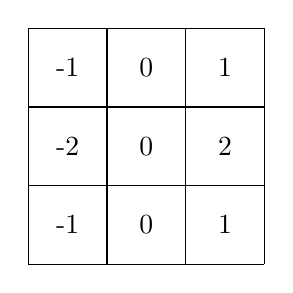
\begin{tikzpicture}
            \draw (0,0) grid (3,3);
            \node at (1-0.5,1-0.5) {-1};
            \node at (1-0.5,2-0.5) {-2};
            \node at (1-0.5,3-0.5) {-1};
            \node at (2-0.5,1-0.5) {0};
            \node at (2-0.5,2-0.5) {0};
            \node at (2-0.5,3-0.5) {0};
            \node at (3-0.5,1-0.5) {1};
            \node at (3-0.5,2-0.5) {2};
            \node at (3-0.5,3-0.5) {1};
        \end{tikzpicture}
    \caption{Edge Detection Convolution Filter}
    \label{fig:Edge Detection Convolution Filter}
\end{figure}



Once the filter is done parsing the image, all the edges are represented by white pixels and everything else is black. More sophisticated techniques like Canny edge detection combine the convolutions step with other steps to find the edges. Figure \ref{fig: Test Room Image} shows the original image and Figure \ref{fig: Test Room Post processed through the Canny edge detector} shows the result obtained after the image is processed through the Canny edge detector.

\begin{figure}[H]
    \centering
    \includegraphics[width=0.8\textwidth]{yo.png}
    \caption{Test Room Image}
    \label{fig: Test Room Image}
\end{figure}

\begin{figure}[H]
    \centering
    \includegraphics[width=0.8\textwidth]{white_edge.png}
    \caption{Test Room Processed Through the Canny Edge Detector}
    \label{fig: Test Room Post processed through the Canny edge detector}
\end{figure}


\subsection{Line Detection}

Line detection is one of the techniques that uses edge detection as its basis, with other techniques built over the edge detection to find the equations of the lines that the edges represent. Advanced methods such as Generalized hough transform can even detect complex shapes like circles or ellipses. Figure \ref{fig: Test Room Processed through Standard Hough Transform} shows the lines detected in Figure \ref{fig: Test Room Image} by one of the more basic methods called the Standard Hough Transform.

\begin{figure}[H]
    \centering
    \includegraphics[width=0.8\textwidth]{white_lines.png}
    \caption{Test Room Processed Through Standard Hough Transform}
    \label{fig: Test Room Processed through Standard Hough Transform}
\end{figure}

\subsection{Corner Detection}

Corner detection is one of the more advanced techniques in computer vision that uses both line and edge detection to find intersection points of edges that also have extreme gradient changes or color changes in multiple directions. Figure \ref{fig: Test Room Processed through Harris Corner Detector} shows all the detected corners in one by using the Harris Corner Detector.

\begin{figure}[H]
    \centering
    \includegraphics[width=0.8\textwidth]{white_corners.png}
    \caption{Test Room Processed Through Harris Corner Detector}
    \label{fig: Test Room Processed through Harris Corner Detector}
\end{figure}

\subsection{Image Segmentation}

Image segmentation is one of the more advanced computer vision techniques, used to find different regions of an image, using multiple steps and methods. The idea is to start with a seed pixel and grow the region based on neighboring pixels. Segmentation works particularly well when used in combination with deep learning techniques, like neural networks.

\subsection{Subject Detection }

Effectively tracking the trajectory of a person within an input video necessitates the continuous detection of the person in each frame and the maintenance of coordinates. Although tracking coordinates in a general image space poses minimal challenges, the transfer of these coordinates to a 3D space introduces complexities. Tackling this task is the main objective of this thesis. However, the first step is to move forward in this problem to effectively detect the subject that will be the main focus in the frame. Neural networks are the most advanced computational models currently available to do this task.

\subsubsection{Neural Networks}

Neural networks are very versatile and complex computational models with various applications and implementations. Computational neural networks are artificially created structures that essentially are supposed to mimic biological neural networks. They consist of nodes and connections. The nodes are supposed to represent the neurons and the edges represent the connections between the neurons. A neural network while mimicking a biological neural network has the structure of a weighted directed graph. A neural network can have a simple linear structure or a very complex structure. However, the information always flows forward like it does in a directed graph.\newline

A simple neural network contains layers of neurons and each layer is completely connected to the next. Each neuron (node) depending on the type of the neural network takes a {0}, {1} value or value between [0,1]. This number is called the activation of the neuron and represents how active the neuron is. That is how much it contributes to the next layer. The activation of the neuron in combination with the weight of the new edge between the node and the next node past trough function called the activation function, and determines how active the next node will be.\newline


\begin{figure}[H]
    \centering
    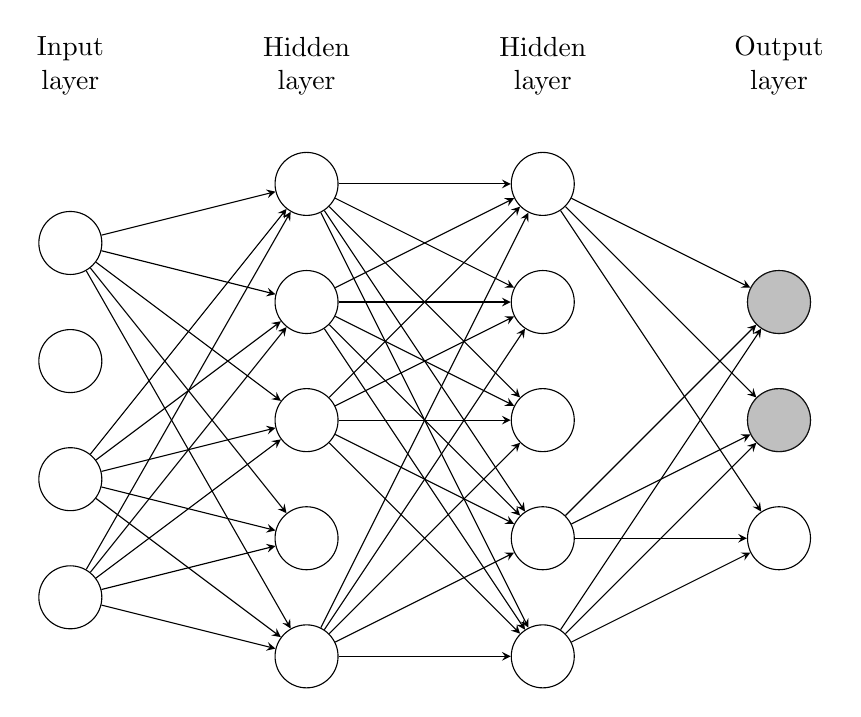
\begin{tikzpicture}[x=1.5cm, y=1.5cm, >=stealth, node distance=2.5cm]
        % Define node style
        \tikzstyle{neuron}=[circle,draw=black,minimum size=8mm]
        
        % Input layer nodes
        \foreach \m/\l [count=\y] in {1,2,3,4}
            \node [neuron] (input-\m) at (-2,2-\y) {};
            
        %Hidden layer nodes
        \foreach \m/\l [count=\y] in {1,2,3,4,5}
            \node [neuron] (hidden1-\m) at (0,2.5-\y) {};
        
        % Second hidden layer nodes
        \foreach \m [count=\y] in {1,2,3,4,5}
            \node [neuron] (hidden2-\m) at (2,2.5-\y) {};
        
        % Output layer nodes
        \foreach \m [count=\y] in {1,2,3}
            \node [neuron] (output-\m) at (4,1.5-\y) {};
        
        \foreach \m [count=\y] in {1,2}
            \node [neuron, fill=black!50, opacity=0.5] (output-\m) at (4,1.5-\y) {};
        
        % Connect input layer with first hidden layer
        \foreach \l [count=\i] in {1,3,4}
            \foreach \j in {1,2,3,4,5}
                \draw [->] (input-\l) -- (hidden1-\j);
        
        % Connect first hidden layer with second hidden layer
        \foreach \l [count=\i] in {1,2,3,5}
            \foreach \j in {1,2,3,4,5}
                \draw [->] (hidden1-\l) -- (hidden2-\j);

        % Connect second hidden layer with output layer
        \foreach \l [count=\i] in {1,4,5}
            \foreach \j in {1,2,3}
                \draw [->] (hidden2-\l) -- (output-\j);

        % Annotate input layer
        \node[align=center] at (-2, 2.5) {Input\\layer};
        
        % Annotate first hidden layer
        \node[align=center] at (0, 2.5) {Hidden\\layer};
        
        % Annotate second hidden layer
        \node[align=center] at (2, 2.5) {Hidden\\layer};
        
        % Annotate output layer
        \node[align=center] at (4, 2.5) {Output\\layer};
    \end{tikzpicture}
    \caption{Neural Network Architecture With Two Hidden Layers}
    \label{fig: Neural Network Architecture with Two Hidden Layers}
\end{figure}

Figure \ref{fig: Neural Network Architecture with Two Hidden Layers} shows a simple neural network. Each node is connected to every node in the next layer. Only the active edges are shown.
Any node that does not have a connection going out of it is inactive. The nodes with a black hue represent the output of the network. We are using Yolo (You Only Look Once) \cite{11}, a widely used neural network in computer vision for the purpose of object detection.\newline

\subsubsection{Pose Detection}

Knowing the orientation that the person is in (sitting, standing, etc.) is particularly important to accurately find the place where they are interacting with the floor, especially in cases where the person is occluded by other objects or is only partially visible in the image space. This can be done by using the proportions of the human body and extending the visible part of the person, according to human body proportions. Google has worked on this and has a tool called Google Media Pipeline \cite{12} which is used in the implementation phase of the solution discussed in the following chapters. 

\subsubsection{Perspective Views}

The 3D world, when projected on a 2D image space, forms a perspective projection, also known as a perspective view. A perspective view is the most accurate representation of how the 3Dimensional world appears from a particular viewpoint. Perspective views are commonly used in computer graphics and engineering to showcase realistic depictions of 3Dimensional objects and scenes. They are often used to render the world in virtual and augmented reality. All images captured by a camera also exist in perspective views. The videos/images obtained from a camera can be in one of three perspectives depending on the orientation of the camera to the surrounding world. The perspectives generally include one vanishing point, two vanishing points, or three vanishing points perspective view. A vanishing point is an imaginary point in the image plane through which all receding parallel lines converge or appear to converge. For each plane in the view that is not orthogonal to the image plane, there exists a vanishing point. Considering a cartesian coordinate system there exist three cardinal planes. In general settings, if we consider one of them to be parallel to the floor and the ceiling, the other two are parallel to the walls of the room/ enclosed space. These three planes contribute to three vanishing points depending on their orientation with the image plane. Objects in the image being captured can exist in planes that are not parallel to any of the cardinal planes and can also have vanishing points of their own leading to cases of more than three vanishing points. Consider being in a cubical room, standing in the centroid of the floor in such a way that you are directly facing the centroid of one of the walls. The view obtained as shown in Figure \ref{fig: One Vanishing point perspective view} would be one vanishing point perspective view.\newline

\begin{figure}[H]
    \centering
    \includegraphics[width=0.9\textwidth]{1vp view.PNG}
    \caption{One Vanishing Point Perspective View}
    \label{fig: One Vanishing point perspective view}
\end{figure}

Now if you rotate to face one of the edges between two walls, the view obtained as shown in Figure \ref{fig: Two Vanishing point perspective view} would be two vanishing point perspective view.\newline

\begin{figure}[H]
    \centering
    \includegraphics[width=0.9\textwidth]{2vp view.PNG}
    \caption{Two Vanishing Point Perspective View}
    \label{fig: Two Vanishing point perspective view}
\end{figure}


Further, if you lift your head to look at the corner, the view obtained would be as shown in Figure \ref{fig: Three vanishing point perspective view} to be three vanishing point perspective view.\newline

\begin{figure}[H]
    \centering
    \includegraphics[width=0.9\textwidth]{3vp view.PNG}
    \caption{Three Vanishing Point Perspective View}
    \label{fig: Three vanishing point perspective view}
\end{figure}


\subsection{Tracking}

The task of following an object or a person through a video stream is known as tracking. In more formal terms, it can be stated as keeping track of a subject whether it is an object or a person through a video stream, as they move through the field of view. Since videos are nothing but consecutive images, finding the coordinates of the subject through of the images and presenting the change all in them with the change in time yields the trajectory of the subject, essentially tracking them. However, looking for the subject in the entire image space is a computationally expensive task but can be made much cheaper to do so. Some techniques that will be used in the next section are discussed as follows.

\subsubsection{Predictive Processing}

The process when a machine, an algorithm, or a living organism makes decisions for the near future by using its knowledge of the world it exists in and its physics by predicting the future based on the current situation is called predictive processing. Humans and animals constantly use predictive processing to interact with the dynamic world around them. Predictive processing is an important part of AI algorithms that interact with the real world, self-driving cars are an example of such an algorithm.

\subsubsection{Feedback Mechanism}

The process by which a system uses its own output to constantly change its state of being is called a feedback mechanism. A feedback mechanism for a system is important for achieving multiple objectives such as maintaining stability, changing the current state to reach a better state, optimizing performance, etc.



\chapter{Methodology}

This chapter will provide a comprehensive solution to the problem statement along with the math required to prove its correctness and to help implement it.\newline

Input: A stream of monocular Images in perspective view with a moving subject.\newline

Output: A trajectory of the subject moving through the image space.\newline

Idea: The idea is to first find the walls, the ceiling, and the floor of the confined space/room. Then, using these walls, Figure out the perspective view that the image exists in and overlay some points on the image as a reference for the coordinate system. Once we have the coordinate system in place, we can start detecting the subject using a neural network. Post detection, we convert the location of the subject from 2D image space to the 3D coordinate system using angular ratios calculated by the extension of projection lines from one of the vanishing points. Continual calculation of these 3D locations yields a trajectory. Further, to make the detection more efficient, we start predicting zones in the image space where the subject might be present in the next frame, and the detection algorithm only looks for the object/person in the predicted zone until the object/person can’t be found or detected in the predicted zone anymore. If the subject is covered by another object, then the focus shifts to the object covering our subject, and we wait for our subject to re-emerge. If the subject does not resurface, the focus shifts back to the entire frame.\newline

We will divide the problem into three subproblems: 1) Mapping the room, 2) Calculating the coordinates of the subject in consideration, and 3) Tracking the subject as he moves through the image space.\newline

\section{Mapping the Room}

To effectively implement the coordinate calculating method proposed further in this chapter, we need to find the vanishing points effectively, and to do so we need to detect the walls and the corners present in the room. Using the edges of the walls to mark the lines on them and extending these lines further, we can calculate the vanishing points. This can be done in a few ways. The first is to use edge detection filters to find all the edges present in the image and draw lines over these edges, further extend these lines to find three line-intersection points, which represent the corners of the room. Using a combination of the lines and the corners to find multiple line intersection points will lead us to the vanishing points. This, however, is a slow and computationally expensive method, and can easily be led in the wrong direction by the presence of other objects in the room, that are not perfectly angular, such as a ball or a chair with a curved back. Another way to do so would be to use image segmentation. Once the wall boundaries are found, we can use a line-detection algorithm to extend the boundaries of the segmented areas and find multiple line-intersection points that represent potential vanishing points. Because segmenting to the ground truth is not easy, there are always errors that occur in the method while finding the exact position of the vanishing point. However, our method helps us to get an area of the image that has a high probability of containing the weighted vanishing point. We can find the centroid of the area that we obtain from the algorithm and use that as the weighted vanishing point. The weighted vanishing point would represent the centroid of all the vanishing points present in the image, depending upon the perspective view of the image.

\section{Calculating the Coordinates}

In this section, we will present and discuss the mathematics required to calculate the coordinates of the subject in 3D spaces.\newline

In the following Figure \ref{fig: Projections from vanishing point} we consider a Vanishing point VP and two subjects along the same line. The subjects have different lengths h and h’ with a common point S somewhere on both the subjects such that the line segment $\overline{VPS}$ is perpendicular to the subjects. We extend projection lines to the endpoints of the subjects from the vanishing point and create projections P and P’ of the subjects at a distance Z’.\newline


\begin{figure}[H]
    \centering
    \includegraphics[width=1.0\textwidth]{Calculations1.jpeg}
    \caption{Projections from Vanishing Point}
    \label{fig: Projections from vanishing point}
\end{figure}

    Considering triangle VPSF1 and VPSF1', we get

    \begin{Equation}[H]
        \begin{equation}
            \label{eq:equation 1}
            \tan(a) + \tan(b) = \frac{h_1}{Z} + \frac{h_2}{Z} = \frac{h}{Z}
        \end{equation}
    \end{Equation}
    
    Considering triangle VPS'B1 and VPS'B1', we get

    \begin{Equation}[H]
        \begin{equation}
        \label{eq:equation 2}
            \tan(a) + \tan(b) = \frac{P_1}{Z} + \frac{P_2}{Z} = \frac{P}{{Z'}}
        \end{equation}
    \end{Equation}
    
    From Eq \ref{eq:equation 1} and Eq \ref{eq:equation 2}

    \begin{Equation}[H]
        \begin{equation}
        \label{eq:equation 3}
            \frac{Z}{Z'} = \frac{h}{P}
        \end{equation}
    \end{Equation}
    
    Similarly, from triangle VPSF2 and VPSF2', and VPS'B2 and VPS'B2'

    \begin{Equation}[H]
        \begin{equation}
        \label{eq:equation 4}
            \tan(a') + \tan(b') = \frac{{h_1'}}{Z} + \frac{{h_2'}}{Z} = \frac{{h'}}{Z}
        \end{equation}
    \end{Equation}
    
    \begin{Equation}[H]
        \begin{equation}
        \label{eq:equation 5}
            \tan(a') + \tan(b') = \frac{{P_1'}}{Z} + \frac{{P_2'}}{Z} = \frac{{P'}}{{Z'}}
        \end{equation}
    \end{Equation}

    From Eq \ref{eq:equation 4} and Eq \ref{eq:equation 5}

    \begin{Equation}[H]
        \begin{equation}
        \label{eq:equation 6}
            \frac{Z}{Z'} = \frac{h'}{P'}
        \end{equation}
    \end{Equation}
    
    From Eq \ref{eq:equation 3} and Eq \ref{eq:equation 6}

    \begin{Equation}[H]
        \begin{equation}
        \label{eq:equation 7}
            \frac{h}{P} = \frac{h'}{P'}
        \end{equation}
    \end{Equation}

\newpage

The following Figure \ref{fig: Generalized Projections from vanishing points} generalizes the angle between $\overline{VPS}$ and the subjects to be T.

\begin{figure}[H]
    \centering
    \includegraphics[width=1.0\textwidth]{Calculations2.jpeg}
    \caption{Generalized Projections from Vanishing Point}
    \label{fig: Generalized Projections from vanishing points}
\end{figure}
    
    From triangle VPSF1'

    \begin{Equation}[H]
        \begin{equation}
        \label{eq:equation 8}
            \cot(a) = \frac{Z + H_1 \cos(T)}{H_1 \sin(T)}
        \end{equation}
    \end{Equation}
    
    From triangle VPS'P1'

    \begin{Equation}[H]
        \begin{equation}
        \label{eq:equation 9}
            \cot(a) = \frac{Z' + P_1 \cos(T)}{P_1 \sin(T)}
        \end{equation}
    \end{Equation}
    
    From Eq \ref{eq:equation 8} and Eq \ref{eq:equation 9}

    \begin{Equation}[H]
        \begin{equation}
        \label{eq:equation 10}
            \frac{Z}{H_1\sin(T)} + \cot(T) = \frac{Z'}{P_1\sin(T)} + \cot(T)
        \end{equation}
    \end{Equation}
    
    Eq \ref{eq:equation 10} can be simplyfied to

    \begin{Equation}[H]
        \begin{equation}
        \label{eq:equation 11}
            \frac{Z}{Z'} = \frac{H_1}{P_1} \quad \text{where } T \neq 0
        \end{equation}
    \end{Equation}
    
    From triangle VPSF1

    \begin{Equation}[H]
        \begin{equation}
        \label{eq:equation 12}
            \cot(b) = \frac{Z - H_2 \cos(T)}{H_2 \sin(T)}
        \end{equation}
    \end{Equation}
    
    From triangle VPS'B1

    \begin{Equation}[H]
        \begin{equation}
        \label{eq:equation 13}
            \cot(b) = \frac{Z' - P_2 \cos(T)}{P_2 \sin(T)}
        \end{equation}
    \end{Equation}
    
    From Eq \ref{eq:equation 12} and Eq \ref{eq:equation 13}

    \begin{Equation}[H]
        \begin{equation}
        \label{eq:equation 14}
            \frac{Z}{H_2\sin(T)} - \cot(T) = \frac{Z'}{P_2\sin(T)} - \cot(T)
        \end{equation}
    \end{Equation}
    
    Eq \ref{eq:equation 14} can be simplyfied to

    \begin{Equation}[H]
        \begin{equation}
        \label{eq:equation 15}
            \frac{Z}{Z'} = \frac{H2}{P2} \quad \text{where } T \neq 0
        \end{equation}
    \end{Equation}
    
    Similarly for a' considering triangles VPSF2' and VPS'P2' and for b' considering triangles VPSF2 and VPSB2 we get,

    \begin{Equation}[H]
        \begin{equation}
        \label{eq:equation 16}
            \cot(a') = \frac{Z + H_1' \cos(T)}{H_1' \sin(T)}
        \end{equation}
    \end{Equation}
    
    \begin{Equation}[H]
        \begin{equation}
        \label{eq:equation 17}
            \cot(a') = \frac{Z' + P_1^{\prime} \cos(T)}{P_1^{\prime} \sin(T)}
        \end{equation}
    \end{Equation}
    
    From Eq \ref{eq:equation 16} and Eq \ref{eq:equation 17}

    \begin{Equation}[H]
        \begin{equation}
        \label{eq:equation 18}
            \frac{Z}{H_1^{\prime}\sin(T)} + \cot(T) = \frac{Z^{\prime}}{P_1^{\prime}\sin(T)} + \cot(T)
        \end{equation}
    \end{Equation}
    
    Simplyfing Eq \ref{eq:equation 18} we get,

    \begin{Equation}[H]
        \begin{equation}
        \label{eq:equation 19}
            \frac{Z}{Z'} = \frac{H_1^{'}}{P_1^{'}} \quad \text{where } T \neq 0
        \end{equation}
    \end{Equation}
    
    From Eq \ref{eq:equation 11} and Eq \ref{eq:equation 19}

    \begin{Equation}[H]
        \begin{equation}
        \label{eq:equation 20}
            \frac{P_1}{H_1} = \frac{P_1^{'}}{H_1^{'}}
        \end{equation}
    \end{Equation}
    
    \begin{Equation}[H]
        \begin{equation}
        \label{eq:equation 21}
            \cot(b') = \frac{Z - H_2^{\prime} \cos(T)}{H_2^{\prime}\sin(T)}
        \end{equation}
    \end{Equation}
    
    \begin{Equation}[H]
        \begin{equation}
        \label{eq:equation 22}
            \cot(b') = \frac{Z' - P_2^{\prime} \cos(T)}{P_2^{\prime}\sin(T)}
        \end{equation}
    \end{Equation}
    
    From Eq \ref{eq:equation 21} and Eq \ref{eq:equation 22}

    \begin{Equation}[H]
        \begin{equation}
        \label{eq:equation 23}
            \frac{Z}{H_2^{\prime}\sin(T)} - \cot(T) = \frac{Z^{\prime}}{P_2^{\prime}\sin(T)} - \cot(T)
        \end{equation}
    \end{Equation}
    
    Simplyfing Eq \ref{eq:equation 23} we get,

    \begin{Equation}[H]
        \begin{equation}
        \label{eq:equation 24}
            \frac{Z}{Z'} = \frac{H_2^{\prime}}{P_2^{\prime}} \quad \text{where } T \neq 0
        \end{equation}
    \end{Equation}
    
    From Eq \ref{eq:equation 15} and Eq \ref{eq:equation 24}

    \begin{Equation}[H]
        \begin{equation}
        \label{eq:equation 25}
            \frac{P_2}{H_2} = \frac{P_2^{\prime}}{H_2^{\prime}}
        \end{equation}
    \end{Equation}
    
    Adding Eq \ref{eq:equation 8} and Eq \ref{eq:equation 12} we get,

    \begin{Equation}[H]
        \begin{equation}
        \label{eq:equation 26}
            \cot(a) + \cot(b) = \frac{Z + H_1 \cos(T)}{H_1 \sin(T)} + \frac{Z - H_2 \cos(T)}{H_2 \sin(T)}
        \end{equation}
    \end{Equation}

    Upon simplification we get,

    \begin{Equation}[H]
        \begin{equation}
        \label{eq:equation 27}
            \cot(a) + \cot(b) = \frac{Z}{\sin(T)} \quad \left(\frac{1}{H_1} + \frac{1}{H_2}\right) = \frac{Z^{\prime}}{\sin(T)} \quad \left(\frac{1}{P_1} + \frac{1}{P_2}\right)
        \end{equation}
    \end{Equation}

    \begin{Equation}[H]
        \begin{equation}
        \label{eq:equation 28}
            \implies \frac{Z}{Z'} = \frac{H_1 H_2 P}{P_1 P_2 H}
        \end{equation}
    \end{Equation}
    
    Similarly for cot(a')+cot(b')

    \begin{Equation}[H]
        \begin{equation}
        \label{eq:equation 29}
            \frac{Z}{Z'} = \frac{(H_1^{\prime} H_2^{\prime}) P^{\prime}}{(P_1^{\prime} P_2^{\prime}) H^{\prime}}
        \end{equation}
    \end{Equation}
    
    Considering Eq \ref{eq:equation 28} and Eq \ref{eq:equation 29}, and using Eq \ref{eq:equation 20} and Eq \ref{eq:equation 25} we get

    \begin{Equation}[H]
        \begin{equation}
        \label{eq:equation 30}
            \frac{H}{P} = \frac{H^{\prime}}{P^{\prime}}
        \end{equation}
    \end{Equation}


From above, considering Figure \ref{fig: Projections from vanishing point} and Figure \ref{fig: Generalized Projections from vanishing points} as references for the calculations, we can see that when considering two objects of different sizes situated at the same place, at point S, if you extend the projection lines from a point, essentially creating projections for both objects at a particular distance, the ratio of the projection to the object, no matter the size of the object, is equal, given that the objects exist both above and below the point. Also, neither of the objects is in line with the projection line passing through point S.\newline

Some other observations can also be made. The ratio of the part of the object above point S to the part of the projection above the projection line through S is equal to the ratio of the object below point S to the part of the projection below the projection line through S. All these ratios—the size of the object to the size of the projection, the size of the parts of the object to the size of the parts of the projection—are also equal to the distance of the vanishing point to point S, and the distance of the vanishing point to the point where the projection line through S intersects the projection (S’).\newline

\begin{figure}[H]
    \centering
    \includegraphics[width=1.0\textwidth]{Calculations3.jpeg}
    \caption{Objects of Different Heights at Different Altitudes}
    \label{fig: Objects of different heights at different altitudes}
\end{figure}

Now consider the Figure \ref{fig: Objects of different heights at different altitudes} for the following\newline

We have three line segments $\overline{U1U2}=U$, $\overline{M1M2} =M$, and $\overline{B1B2} =B$ on the same line, and their projections $\overline{U1'U2'}=U'$, $\overline{M1'M2'} =M'$ and $\overline{B1'B2'}=B'$ on the same line $\overline{U1U2}$ and $\overline{B1B2}$ do not overlap, whereas $\overline{M1M2}$ has an overlap with both $\overline{U1U2}$ and $\overline{B1B2}$. That is also true for their projections using the observations from the previous sections. We can see that U'/U=S1'/S1=M'/M, B'/B=S2'/S2=M'/M, Hence, U'/U=B'/B=S1'/S1=S2'/S2.\newline

We can infer a few things from the above sections. The ratios of the line segments to the projections are equal, even though they do not intersect, as long as the line segments and their projections exist on the same lines, respectively. The ratio that we obtain is also independent of the length of the line segment as any change in the length of the line segment is also reflected in the projection. Now combining this information with the information that we have about the world in perspective view images, all parallel lines, depending on the number of vanishing points and the orientation of the parallel lines with respect to the vanishing point, either converge to a vanishing point in the image space or are parallel to each other in the image space. Either way, any object situated at a particular point, no matter its size or altitude from the floor, will be on the same line in the image space as in the real world. It will exist on the same Z coordinate, and that Z coordinate like all other Z coordinates will translate to a line passing through one of the vanishing points or a line parallel to all other Z coordinates.\newline

If we can standardize the positioning of the projection, we will obtain a standardized depth estimating system, which in combination with an absolute step size definition can be used to calculate and obtain the position/coordinates of the object/person.\newline

When a person is moving he typically remains in contact with the floor (i.e. walking or running). Knowing when the person is not on the floor (i.e. jumping) requires the method to have a comprehensive and nuanced grasp of various factors and details such as contextual clues, body movements, environmental interactions, etc. Since, doing so in a monocular image with no extra information is it a difficult and computationally expensive task and only covers a minor portion of the cases, we will assume that the person is always in contact with the floor.\newline

Consider the projection lines, passing through the bottom of the subject and extend the line to reach the bottom line of the image $\overline{VP}$. As shown above, we only need the distance of the bottom of the subject from the projection point $\overline{VT}$ and the distance of the projection from the projection point $\overline{VP}$ i.e. the bottom line of the image from the projection point, measured along the projection line. We take the ratio of two and call it to be F as shown in Figure \ref{fig: Ratios on the floor}.\newline

\begin{figure}[H]
    \centering
    \includegraphics[width=1.0\textwidth]{Calculations4.jpeg}
    \caption{Ratios on The floor}
    \label{fig: Ratios on the floor}
\end{figure}

    \begin{Equation}[H]
        \begin{equation}
        \label{eq:equation 31}
            \overline{VT} = S
        \end{equation}
    \end{Equation}
    
    \begin{Equation}[H]
        \begin{equation}
        \label{eq:equation 32}
            \overline{VP} = S'
        \end{equation}
    \end{Equation}
    
    \begin{Equation}[H]
        \begin{equation}
        \label{eq:equation 33}
            F = \frac{S}{S'} = \frac{\overline{VT}}{\overline{VP}}
        \end{equation}
    \end{Equation}


We further need a standardized point to extend the projection lines from. There are a few options that we can consider. The first would be to use the vanishing points, but depending upon the view angle and the positioning of the room, there can be multiple vanishing points. Choosing different points would give different coordinates for people/objects. The second option to tackle would be to consider a point that accounts for all the vanishing points. In the case of one vanishing point perspective view, that would be the vanishing point itself. In the case of two vanishing point perspective view, it would be the center of the line joining both of the vanishing points. And in the case of the three vanishing point perspective view, it would be the centroid of the triangle formed by the three vanishing points. The third option would be to consider the center of the image frame. This works on the same idea as the other two cases, requires the least calculations, and is the easiest to implement; however, it is prone to errors.\newline

If the center of the image is chosen to be the projection point, and the positioning of the camera and the room are at an extreme position/angle to each other. There can be cases where the floor crosses the center of the image frame, which will lead to some errors because at that point there can be a subject that is placed directly at the projection point and our calculations for that subject will indicate that they are standing at infinity, which would be wrong. Such a scenario can be avoided by using the second option, which encapsulates the idea of using all of the vanishing points and will always yield the correct results.\newline

The next step in the problem is to define an absolute origin. For our coordinate system, we again have a few options to consider. We could use the projection point as the origin, but since it is supposed to be a representation of the vanishing points, it is infinitely far from the image plane and will place all the objects in consideration at infinity. The second option is to place the origin at one of the corners of the room. At first, this feels intuitive and would make translating the coordinates to the real world easy, which helps open more practical use cases. However, calculating the coordinates of the subject, with respect to a separate point as compared to one not directly related to the point being used to calculate the depth of the person requires additional calculations at each step. The third option—to place the origin—would be to consider a point that relates to the projection point, and one that is close enough to the image plane. Hence, we can project the point directly to the bottom of the image and consider the point at the floor that the projection corresponds to, to be our origin. We can then calculate the position of all the people/objects in consideration with respect to this, the coordinates of the corners, and the walls can also be calculated using the same logic. After calculation, if needed, the original can be shifted to any one of these corners of the room by simply translating and rotating the coordinate system. Depending on the camera placement\newline

Now that we have the origin in place, the next step is to turn the ratio that we have corresponding to the depth into absolute Z coordinates. To do so we still need to define a step size in terms of the image space this can be defined either in terms of an absolute number of pixels add the image plane, or as a factor of the dimensions of the image which can then be translated to a number of pixels. Figure \ref{fig:Step Size} Shows the step size at the image plane, Figure \ref{fig: Step Size label} focuses on the bottol left half of the room in Figure \ref{fig:Step Size} and provides labels for the step size and the projection point.\newline

\begin{figure}[H]
    \centering
    \includegraphics[width=1.0\textwidth]{Calculations5.jpeg}
    \caption{Step Size}
    \label{fig:Step Size}
\end{figure}

\begin{figure}[H]
    \centering
    \includegraphics[width=1.0\textwidth]{Calculations6.jpeg}
    \caption{Step Size Labels}
    \label{fig: Step Size label}
\end{figure}

Considering following Figure $\ref{fig: Support for depth calculation}$ we can assume the step size at the image plane to be A and the distance from the projection point to the base of the image plan projected on the image to be S as the projection point is at infinity, there needs to be infinite steps, each of step size a taken to reach it, all the steps are represented in S and are gradually getting smaller and smaller. This can be represented as an infinitely decreasing geometric progression whose first term is a and the sum is S using these two values we can calculate the common ratio r of the geometric progression.\newline

By convention, we will consider S to be the distance between the projection point, and the bottom corner of the image which is further from the projection point.\newline

\begin{figure}[H]
    \centering
    \includegraphics[width=1.0\textwidth]{Calculations7.jpeg}
    \caption{Support for Depth Calculation}
    \label{fig: Support for depth calculation}
\end{figure}

\begin{Equation}[H]
        \begin{equation}
        \label{eq:equation 34}
            S = \frac{A}{1 - r}
        \end{equation}
    \end{Equation}
    
    \begin{Equation}[H]
        \begin{equation}
        \label{eq:equation 35}
        \implies 1 - r = \frac{A}{S}
        \end{equation}
    \end{Equation}
    
    \begin{Equation}[H]
        \begin{equation}
        \label{eq:equation 36}
        \implies r = 1 - \left(\frac{A}{S}\right) \quad \text{where } S > A
        \end{equation}
    \end{Equation}

\begin{figure}[H]
    \centering
    \includegraphics[width=1.0\textwidth]{Calculations8.jpeg}
    \caption{Support for Depth Calculation}
    \label{fig: Support for depth calculation labels}
\end{figure}

Figure \ref{fig: Support for depth calculation} shows a room with projection line extend form the projection point, and Figure \ref{fig: Support for depth calculation labels} focuses on the bottom right quarter of the image and provides labels to support the following calculations.\newline

Now, for a person at a certain depth with the projection at the image plane as X, we take n steps to reach the depth, as X is the sum of n steps that are part of a geometric progression we can calculate n as follows.\newline


\begin{Equation}[H]
        \begin{equation}
        \label{eq:equation 37}
            X = \frac{A(1 - r^n)}{1 - r}
        \end{equation}
    \end{Equation}
    
    \begin{Equation}[H]
        \begin{equation}
        \label{eq:equation 38}
        \implies \frac{X(1 - r)}{A} = 1 - r^n
        \end{equation}
    \end{Equation}
    
    \begin{Equation}[H]
        \begin{equation}
        \label{eq:equation 39}
        \implies r^n = 1 - \frac{X(1 - r)}{A}
        \end{equation}
    \end{Equation}
    
    \begin{Equation}[H]
        \begin{equation}
        \label{eq:equation 40}
        \implies r^n = 1 - \frac{X}{S} \quad \text{where } S = \frac{A}{1 - r} \text{ From Eq \ref{eq:equation 34}}
        \end{equation}
    \end{Equation}
    
    Taking log on both sides

    \begin{Equation}[H]
        \begin{equation}
        \label{eq:equation 41}
             n \log(r) = \log\left(1 - \frac{X}{S}\right)
        \end{equation}
    \end{Equation}
    
    \begin{Equation}[H]
        \begin{equation}
        \label{eq:equation 42}
        \implies n = \frac{\log\left(1 - \frac{X}{S}\right)}{\log(r)}
        \end{equation}
    \end{Equation}
    
    \begin{Equation}[H]
        \begin{equation}
        \label{eq:equation 43}
        \implies n = \log_r(F)
        \end{equation}
    \end{Equation}
    
    \begin{Equation}[H]
        \begin{equation}
        \label{eq:equation 44}
            F = 1 - \frac{X}{S}
        \end{equation}
    \end{Equation}


Here F is nothing but the ratio of the distance of the subject from the projection point to the distance of the projection of the site subject from the projection point calculated along the projection line. Calculation of F was also discussed in the previous sections. This ratio can also be written as the ratio of the y coordinates of the points due to triangle similarity. We consider the coordinates of the Vanishing point to be (X,Y) and the coordinates of the subject to be (x,y)\newline

\begin{Equation}[H]
    \begin{equation}
    \label{eq:equation 45}
        F = 1 - \frac{Y-y}{Y}
    \end{equation}
\end{Equation}

\begin{figure}[H]
    \centering
    \includegraphics[width=1.0\textwidth]{Calculations9.jpeg}
    \caption{Coordinate System}
    \label{fig: Coordinate System}
\end{figure}

Figure \ref{fig: Coordinate System} Shows the Projection point O, the origin O’, and a person represented by the lime P. In the figure, the line connecting the origin to the projection point OO' is given by x= y=0.\newline

The following Figures, Figure \ref{fig: Medium sized object}, Figure \ref{fig: Tall person}, and Figure \ref{fig: Extremely small object}, show one of the more extreme angle placements of the camera relative to the scene. All images have been clicked from the same camera angle and show subjects of different heights standing at the same position in the real world. P represents the projection point and is also the centroid of all the vanishing points, the point on the floor where the subject stands is represented by Z and the point of intersection of the projection line with the image edge is Z’. Since the camera is not moving P is the same and because the subjects all stand at the same point Z for all three is also the same, hence the the ratio $\overline{PZ}$/$\overline{PZ’}$ is the same in all three cases resulting in the same coordinates.\newline

\begin{figure}[H]
    \centering
    \includegraphics[width=0.9\textwidth]{3vpmo.jpeg}
    \caption{Medium Sized Object}
    \label{fig: Medium sized object}
\end{figure}

\begin{figure}[H]
    \centering
    \includegraphics[width=0.8\textwidth]{3vpto.jpeg}
    \caption{Tall Person}
    \label{fig: Tall person}
\end{figure}

\begin{figure}[H]
    \centering
    \includegraphics[width=0.8\textwidth]{3vpso.jpeg}
    \caption{Extremely Small Object}
    \label{fig: Extremely small object}
\end{figure}

\section{Tracking}

After the coordinates of any subject have been calculated in one frame, we only need to continuously detect them in consecutive frames. The accuracy and the precision of the detection depend on the model being used to detect the subject for testing. we are using Yolo as it provides a high accuracy whilst being light enough to be run on most devices locally. However, looking at the entire image space in each frame can be computationally expensive. Therefore, we will implement some techniques to reduce the computation cost and make the overall algorithm faster.\newline

The aim is to mimic the way that living organisms track objects moving through their field of view. The idea is to create a small dynamic window around the object/person once they are detected and then use predictive programming to predict where the person might be in the next frame And move the window to the predicted place of the image space. We keep buffer space around the person and use the coordinates of the subject within the image space from the past few frames to calculate the average speed and the direction of motion of the subject to estimate their position in the next frame. we also create a feedback globe as each time the set of past frames being used to calculate the position is updated. The size of the buffer can also be changed, depending upon the speed of the subject, and the window can be skewed in the direction of the motion.\newline


\chapter{Implementation and Results}

This chapter aims to provide a high-level algorithm that can be used to implement the solution provided in the previous Chapter. We will also present and discuss the results achieved from the implementation of the proposed method. Before moving forward let us reiterate the problem statement. There exists a gap in research for methods to track objects or people in 3D space that needs no pre-preparation or a lot of special equipment to gather data. the aim of this thesis is to find that requires neither of those two things and can work on a monocular RGB vision image or video, captured by a regular phone camera.\newline

The idea to solve this is to use the vanishing points existing in the space to Figure out the depth of the subject in consideration and continue tracking of the coordinates found using the depth gives the trajectory of the person as they move through the image space. so we first need to Figure out where the vanishing points lie in the space, and then we need to find the boundaries of the walls present in the scene then using the method proposed in the previous chapter, we find the coordinates of the subject and do this over and over for each new frame essentially tracking them.\newline

\section{Implementation}

The idea for the implementation is rather simple We divide the task into 2 parts, the first is to find the weighted vanishing point, and the second is to calculate the 3D coordinate of the subject.\newline

\subsection{Weighted Vanishing Point}

The idea behind finding the weighted vanishing point is to start with the frame and run an edge detection filter over it to get an edge map of the image algorithm \ref{Edge Detection Algorithm (Part 1)} and algorithm \ref{Edge Detection Algorithm (Part 2)} present the idea to do so. Once we have the edge map of the image we find all the lines present in the image. To do so we generate lines with slopes ranging from 0 to $\pi$ and then pass them over and through the edge map and check if a minimum threshold for the length overlap with the line if yes we add the line to a set, algorithm \ref{Line Overlay Algorithm (Part 1)} and algorithm \ref{Line Overlay Algorithm (Part 2)} implement this idea. We then find points that have more than T’ lines passing through them, T’ is the threshold for a point to be considered a Vanishing Point we then take the centroid of all the points and that is our weighted vanishing point, algorithm \ref{Weighted Vanishing Point Algorithm} implements this idea to calculate the coordinates of the weighted vanishing point.

\begin{algorithm}[H]
    \label{Edge Detection Algorithm  (Part 1)}
\setstretch{1.0}

\SetAlgoLined
    \SetKwInOut{Input}{Input}
    \SetKwInOut{Output}{Output}
    
    \Input{Image as an $m \times n$ matrix}
    \Output{Edge map of the image as an $m \times n$ matrix}
    $T \leftarrow$ Threshold\;
    Gradient map $\leftarrow$ $m \times n$ matrix\;
    Edge map $\leftarrow$ $m \times n$ matrix\;
    
    \For{$i \leftarrow 1$ \KwTo $n$}{
        \For{$j \leftarrow 1$ \KwTo $m$}{
            $gx \leftarrow (a_{i-1,j+1} - a_{i-1,j-1}) + 2 (a_{i,j+1}-a_{i,j-1}) + (a_{i+1,j+1} - a_{i+1,j-1})$\;
            $gy \leftarrow (a_{i+1,j-1} - a_{i-1,j-1}) + 2 (a_{i+1,j}-a_{i-1,j}) + (a_{i+1,j+1} - a_{i-1,j+1})$\;
            $\text{gradient magnitude} \leftarrow \sqrt{gx^2+gy^2}$\;
            $\text{gradient direction} \leftarrow \arctan{\frac{gx}{gy}}$\;
            $\text{Gradient map}_{i,j} \leftarrow (\text{gradient magnitude}, \text{gradient direction})$\;
        }
    }

    \caption{Edge Detection Algorithm  (Part 1)}
\end{algorithm}

\newpage


\begin{algorithm}[H]
    \label{Edge Detection Algorithm  (Part 2)}
\setstretch{1.0}

\SetAlgoLined

\setcounter{AlgoLine}{12}

    \For{$i \leftarrow 1$ \KwTo $n$}{
        \For{$j \leftarrow 1$ \KwTo $m$}{
            $\text{angle} \leftarrow \text{gradient direction}_{i,j}$\;
            \If{$\text{gradient magnitude}_{i,j} \geq T$}{
                \If{$-22.5 \leq \text{angle} < 22.5$ or $\text{angle} \geq 157.5$ or $\text{angle} < -157.5$}{
                    \If{$\text{gradient magnitude}_{i,j} \geq \text{gradient magnitude}_{i,j-1}$ and $\text{gradient magnitude}_{i,j} \geq \text{gradient magnitude}_{i,j+1}$}{
                        $\text{Edge map}_{i,j} \leftarrow 1$\;
                    }
                }
                \ElseIf{$22.5 \leq \text{angle} < 67.5$ or $-157.5 \leq \text{angle} < -112.5$}{
                    \If{$\text{gradient magnitude}_{i,j} \geq \text{gradient magnitude}_{i - 1,j + 1}$ and $\text{gradient magnitude}_{i,j} \geq \text{gradient magnitude}_{i + 1,j - 1}$}{
                        $\text{Edge map}_{i,j} \leftarrow \text{gradient magnitude}_{i,j}$\;
                    }
                }
                \ElseIf{$67.5 \leq \text{angle} < 112.5$ or $-112.5 \leq \text{angle} < -67.5$}{
                    \If{$\text{gradient magnitude}_{i,j} \geq \text{gradient magnitude}_{i - 1,j}$ and $\text{gradient magnitude}_{i,j} \geq \text{gradient magnitude}_{i + 1,j}$}{
                        $\text{Edge map}_{i,j} \leftarrow \text{gradient magnitude}_{i,j}$\;
                    }
                }
                \ElseIf{$112.5 \leq \text{angle} < 157.5$ or $-67.5 \leq \text{angle} < -22.5$}{
                    \If{$\text{gradient magnitude}_{i,j} \geq \text{gradient magnitude}_{i - 1,j - 1}$ and $\text{gradient magnitude}_{i,j} \geq \text{gradient magnitude}_{i + 1,j + 1}$}{
                        $\text{Edge map}_{i,j} \leftarrow \text{gradient magnitude}_{i,j}$\;
                    }
                }
            }
        }
    }
    \Return Edge map
    \caption{Edge Detection Algorithm (Part 2)}
\end{algorithm}
    
\newpage
    
    
    
\begin{algorithm}[H]
    \label{Line Overlay Algorithm (Part 1)}
\setstretch{1.0}

\SetAlgoLined
\SetKwInOut{Input}{Input}
\SetKwInOut{Output}{Output}

\Input{Edge map of the image}
\Output{Set of lines overlaying the edge map}
lines $\leftarrow \{\}$\;
$L \leftarrow$ Threshold for minimum length\;
    
    \For{$i\leftarrow 0$ \KwTo $n-1$}{
        $\theta \leftarrow \arctan(\frac{m}{n-i})$\;
        $\Omega \leftarrow \arctan(\frac{m}{i-n}$)\;
        \For{$x'\leftarrow 0$ \KwTo $n$}{
            line $\leftarrow y=\theta(x-x')$\;
            $P=\{P_1,\dots,P_k\}$ \tcp*[r]{Points on the line}
            \For{$j\leftarrow 1$ \KwTo $k-L$}{
                \If{$\sum_{a=1}^{j+L} P_a = L$}{
                    lines $\leftarrow$ line\;
                }
            }
            line $\leftarrow y=\omega(x-x')$\;
            $P=\{P_1,\dots,P_k\}$
            \For{$j\leftarrow 1$ \KwTo $k-L$}{
                \If{$\sum_{a=1}^{j+L} P_a = L$}{
                    lines $\leftarrow$ line\;
                }
            }
        }
    
        
        \For{$y'\leftarrow 0$ \KwTo $m$}{
            line $\leftarrow (y-y')=\theta(x)$\;
            $P=\{P_1,\dots,P_k\}$
            \For{$j\leftarrow 1$ \KwTo $k-L$}{
                \If{$\sum_{a=1}^{j+L} P_a = L$}{
                    lines $\leftarrow$ line\;
                }
            }
            line $\leftarrow (y-y')=\omega(x-m)$\;
            $P=\{P_1,\dots,P_k\}$
            \For{$j\leftarrow 1$ \KwTo $k-L$}{
                \If{$\sum_{a=1}^{j+L} P_a = L$}{
                    lines $\leftarrow$ line\;
                }
            }
        }
    }
\caption{Line Overlay Algorithm (Part 1)}
\end{algorithm}


\newpage

\begin{algorithm}[H]
    \label{Line Overlay Algorithm (Part 2)}
\setstretch{1.0}

\SetAlgoLined

\setcounter{AlgoLine}{38}

\SetKwInOut{Input}{Input}
\SetKwInOut{Output}{Output}

    \For{$i\leftarrow 0$ \KwTo $m$}{
        $\theta \leftarrow \arctan(\frac{m-1}{n})$\;
        $\Omega \leftarrow \arctan(\frac{i-m}{n})$\;
        \For{$x'\leftarrow 0$ \KwTo $n$}{
            line $\leftarrow y=\theta(x-x')$\;
            $P=\{P_1,\dots,P_k\}$ \tcp*[r]{Points on the line}
            \For{$j\leftarrow 1$ \KwTo $k-L$}{
                \If{$\sum_{a=1}^{j+L} P_a = L$}{
                    lines $\leftarrow$ line\;
                }
            }
            line $\leftarrow y=\omega(x-x')$\;
            $P=\{P_1,\dots,P_k\}$
            \For{$j\leftarrow 1$ \KwTo $k-L$}{
                \If{$\sum_{a=1}^{j+L} P_a = L$}{
                    lines $\leftarrow$ line\;
                }
            }
        }
    
        
        \For{$y'\leftarrow 0$ \KwTo $m$}{
            line $\leftarrow (y-y')=\theta(x)$\;
            $P=\{P_1,\dots,P_k\}$
            \For{$j\leftarrow 1$ \KwTo $k-L$}{
                \If{$\sum_{a=1}^{j+L} P_a = L$}{
                    lines $\leftarrow$ line\;
                }
            }
            line $\leftarrow (y-y')=\omega(x-m)$\;
            $P=\{P_1,\dots,P_k\}$
            \For{$j\leftarrow 1$ \KwTo $k-L$}{
                \If{$\sum_{a=1}^{j+L} P_a = L$}{
                    lines $\leftarrow$ line\;
                }
            }
        }
    }
    
    \Return lines
    
\caption{Line Overlay Algorithm (Part 2)}
\end{algorithm}

\newpage


\begin{algorithm}[H]
    \label{Weighted Vanishing Point Algorithm}
\setstretch{1.0}

\SetAlgoLined
\SetKwInOut{Input}{Input}
\SetKwInOut{Output}{Output}

\Input{A set of lines}
\Output{Coordinates of the weighted vanishing point}
$T \leftarrow$ Threshold for line intersection\;
Points $\leftarrow \{\}$\;

    \For{$j \leftarrow i$ \KwTo $n-1$}{
        \For{$k \leftarrow i+1$ \KwTo $n$}{
            $x = \frac{(m_j \cdot x_j \cdot m_k \cdot x_k) + (y_k - y_j)}{(m_j - m_k)}$\;
            $y = m_j \cdot (x - x_j) + y_j$\;
            \If{$(x,y)$ in Points}{
                Increment count of $(x,y)$ in Points\;
            }
            \Else{
                Add $(x,y)$ to Points with count 1\;
            }
        }
    }
    
    \For{$P_i$ in Points}{
        \If{count of $P_i < T$}{
            Remove $P_i$ from Points\;
        }
    }
    
    $X = \frac{\sum_{i=1}^{n} x_i}{n}$\;
    $Y = \frac{\sum_{i=1}^{n} y_i}{n}$\;
    
    \Return{Weighted vanishing point: $(X,Y)$}
    \caption{Weighted Vanishing Point Algorithm}
    \end{algorithm}
    
    \newpage

    \subsection{Coordinate Calculation}

    In this subsection, we will provide an algorithm to implement the idea discussed in Chapter 4 to calculate the 3D coordinate of the subject if we have the coordinate of the subject in the image space, the weighted vanishing point in the image space, and the step size.\newline

    The idea is to calculate the number of steps required to reach the depth of the subject and then calculate the step size at that depth and then calculate the position of the subject relative to the origin in 3D space. The following algorithm \ref{3D Coordinates Calculation Algorithm} implements this idea.\newline
    
    \begin{algorithm}[H]
        \label{3D Coordinates Calculation Algorithm}
    \setstretch{1.0}
    \SetAlgoLined
    \SetKwInOut{Input}{Input}
    \SetKwInOut{Output}{Output}
    
    \Input{Position of the subject $(x,y)$ in the image space, coordinates of the weighted vanishing point $(X,Y)$, Step Size $A$}
    \Output{Coordinates of the person in 3D space $(x',0,z)$}
    
    $z \leftarrow$ Depth\;
    $r \leftarrow 1 - \frac{A}{\sqrt{X^2+Y^2}}$\;
    $r^n \leftarrow 1 - \frac{Y-y}{Y}$\;
    $n \leftarrow \log_r(r^n)$ \tcp*[r]{Number of steps to reach the depth}
    $z \leftarrow n$\;
    $x' \leftarrow \frac{(x-X)}{A \cdot r^n}$\;
    
    \Return{$(x',0,z)$} \tcp*[r]{Subject assumed to be on the floor}
    \caption{3D Coordinates Calculation Algorithm}
    \end{algorithm}
    
    



\section{Results}

In this section, we will discuss the experimental setup and the results obtained at each step of the implementation of the method.\newline

\subsection{The Experimental Setup}

For our experimental setup, we have monocular images of different places in different perspective views, we also have monocular video streams In different orientations and perspective views. These images are then processed in Python to obtain the results which are shown in the sections that follow.\newline

\subsection{Mapping the Room}

To map the room effectively we essentially need to find the corners and the edges of the walls and then using the Contextual information that can be extracted from the walls and the floor and the roof of the room Figure out the perspective view that the image exists in. further we need to Figure out the centroid of the vanishing points.\newline

Some methods that can be used to do so are edge detection filters, line detection algorithms, corner detection algorithms, and image segmentation models, for our testing we have used image segmentation along with these other techniques to Figure out the weighted vanishing point, or in other words the centroid of the vanishing point.\newline

\begin{figure}[H]
    \centering
    \includegraphics[width=1.0\textwidth]{1vp room.jpg}
    \caption{A Room in 1VP Perspective View}
    \label{fig: A room in 1VP perspective view}
\end{figure}


Figure \ref{fig: A room in 1VP perspective view} and Figure \ref{fig: A room in 3VP perspective view} represent two rooms in 1VP perspective view and 3VP prespective view respectively. These images are passed through an image segmentation algorithm to detect walls. Figure \ref{fig: 1VP perspective view room segmentation} and Figure \ref{fig: 3VP perspective view room segmentation}  showcase the result obtained from the segmentation algorithm. The boundary marked in green is the segmentation boundary.\newline

\begin{figure}[H]
    \centering
    \includegraphics[width=1.0\textwidth]{1vp Segmentation Result.png}
    \caption{1VP Perspective View Room Segmentation}
    \label{fig: 1VP perspective view room segmentation}
\end{figure}

\begin{figure}[H]
    \centering
    \includegraphics[width=1.0\textwidth]{1vp Segmentation and Corner Detection Result.png}
    \caption{1VP Perspective View Line Detection}
    \label{fig: 1VP perspective view line detection}
\end{figure}

Figure \ref{fig: 1VP perspective view line detection} and Figure \ref{fig: 3VP perspective view line detection} show the lines marked using the segmentation boundaries. As Figure \ref{fig: A room in 1VP perspective view} to Figure \ref{fig: 1VP perspective view Weighted Vanishing Point} represent a rather simple scene it is easy to see that most of the lines marked with the help of the segmentation boundary lead to the centre of the image which also is the only vanishing point. However, for more complex scenes such as the one presented in Figure 5-8 to Figure 5-12, it is not that easy to see the vanishing points.\newline

\begin{figure}[H]
    \centering
    \includegraphics[width=1.0\textwidth]{1vp Most Converged Area.png}
    \caption{1VP Perspective View Vanishing Point Possibility Space}
    \label{fig: 1VP perspective view Vanishing point possibility space}
\end{figure}

Figure Figure \ref{fig: 1VP perspective view Vanishing point possibility space} and Figure \ref{fig: 3VP perspective view Vanishing point possibility space} show the area that has points where multiple lines intersect, it is important to note that a lot of these points don’t neceseraly have receding parallel lines intersecting at them, but lines that are orthogonal to the vanishing points. Because these are not special points they are distrtributed over the entire image space and don’t really contribute in finding the weighted vanishing point.\newline

\begin{figure}[H]
    \centering
    \includegraphics[width=1.0\textwidth]{1vp Centroid of Most Converged Area.png}
    \caption{1VP Perspective View Weighted Vanishing Point}
    \label{fig: 1VP perspective view Weighted Vanishing Point}
\end{figure}

Figure \ref{fig: 1VP perspective view Weighted Vanishing Point} and Figure \ref{fig: 3VP perspective view Weighted Vanishing Point} Show the weighted vanishing point that can later be used to calculate the ratios and further the depth and coordinates of the people/objects present in the scene.\newline

\begin{figure}[H]
    \centering
    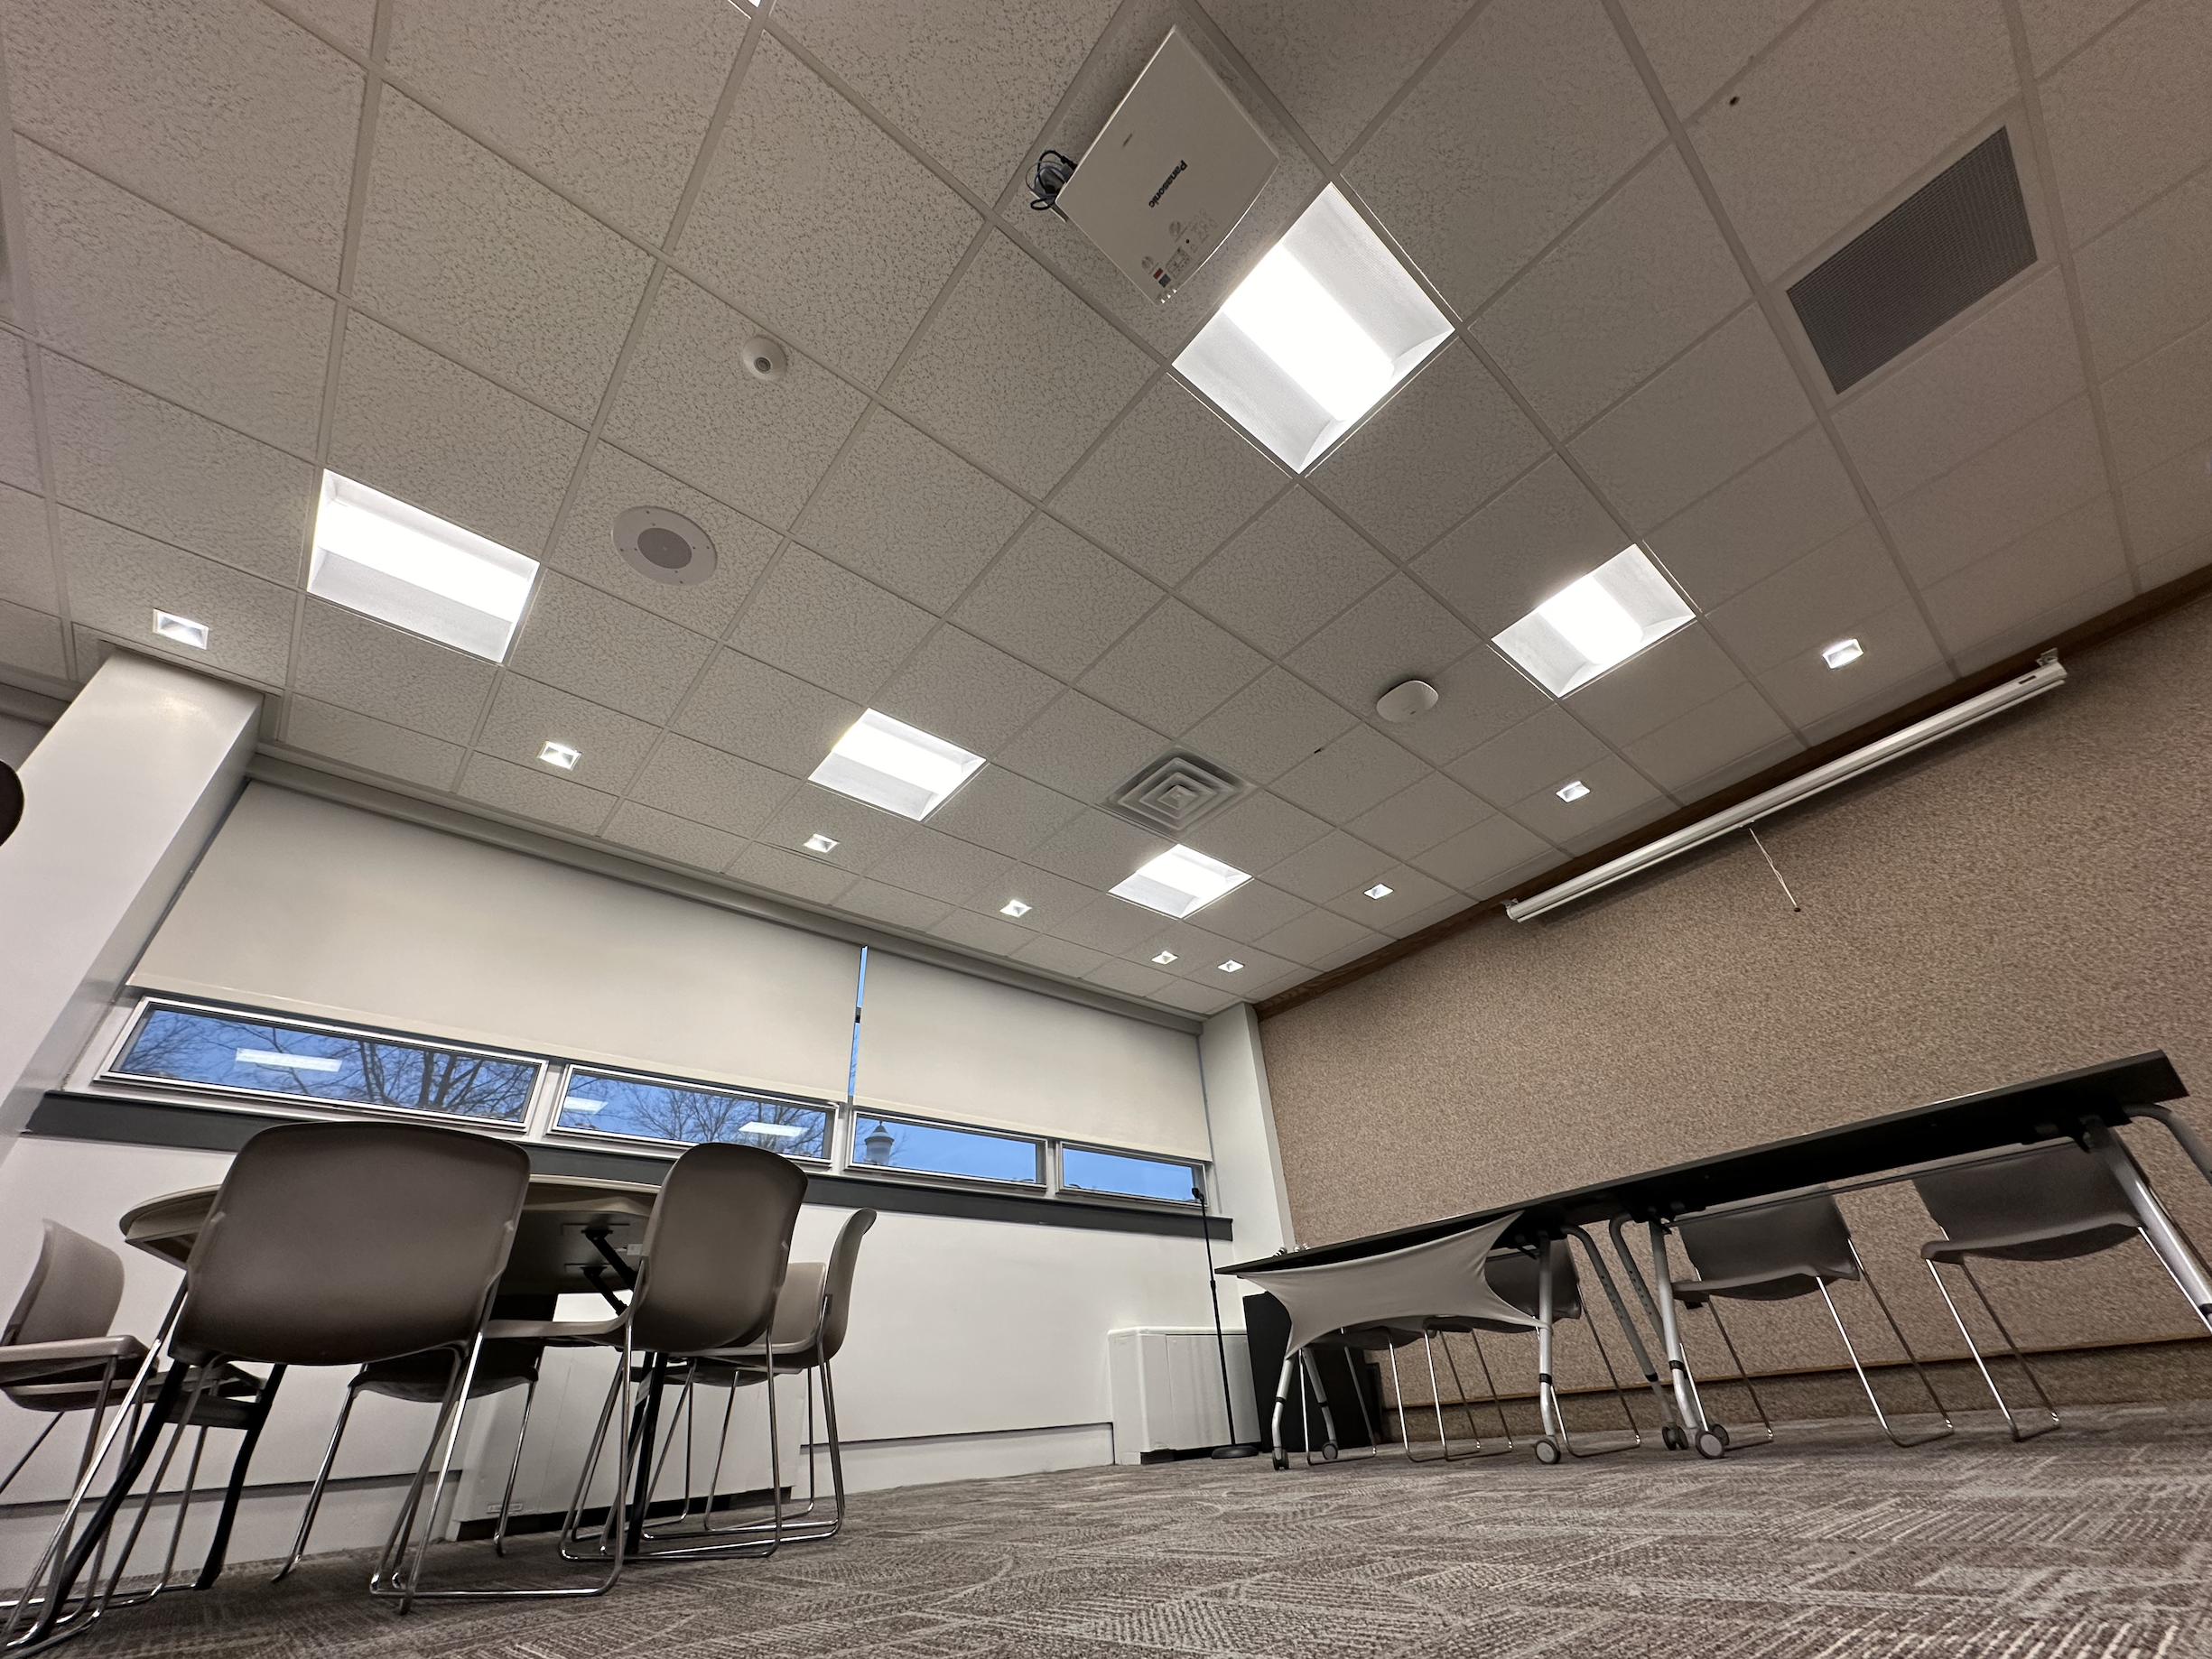
\includegraphics[width=0.8\textwidth]{3vp.png}
    \caption{A Room in 3VP Perspective View}
    \label{fig: A room in 3VP perspective view}
\end{figure}

\begin{figure}[H]
    \centering
    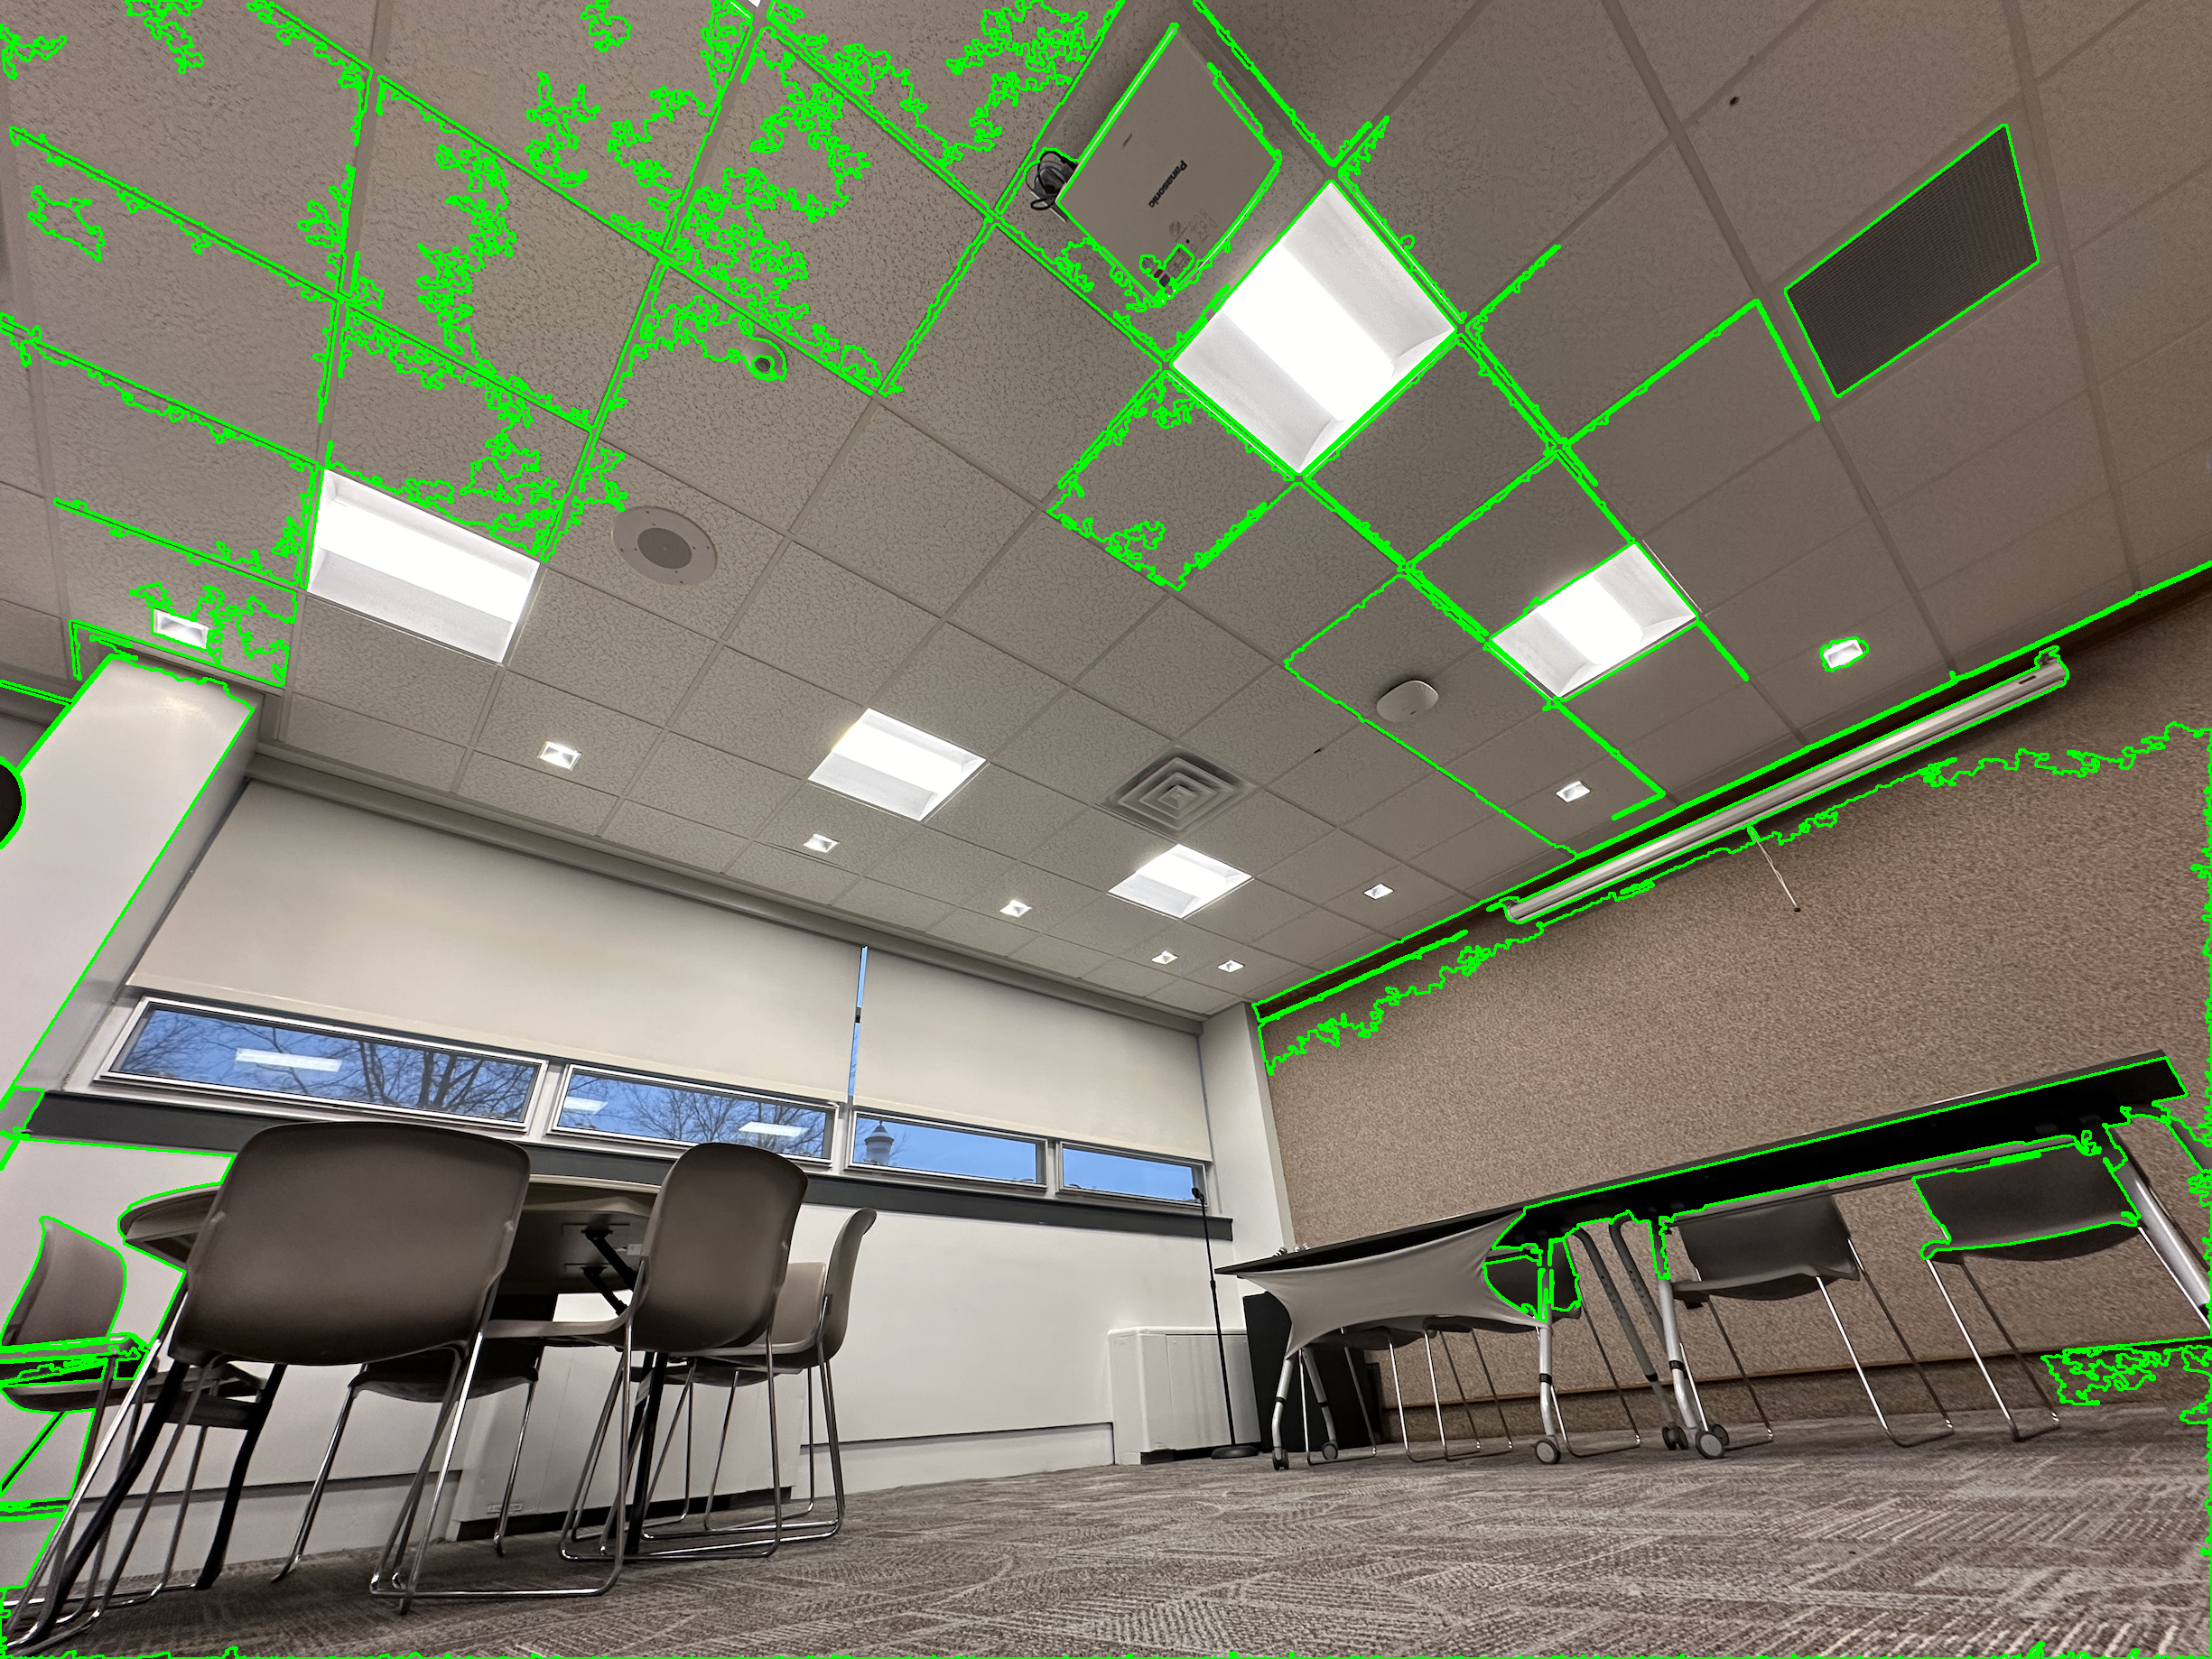
\includegraphics[width=0.8\textwidth]{3vp Segmentation Result.png}
    \caption{3VP Perspective View Room Segmentation}
    \label{fig: 3VP perspective view room segmentation}
\end{figure}

\begin{figure}[H]
    \centering
    \includegraphics[width=0.8\textwidth]{3vp Segmentation and Corner Detection Result.png}
    \caption{3VP Perspective View Line Detection}
    \label{fig: 3VP perspective view line detection}
\end{figure}

\begin{figure}[H]
    \centering
    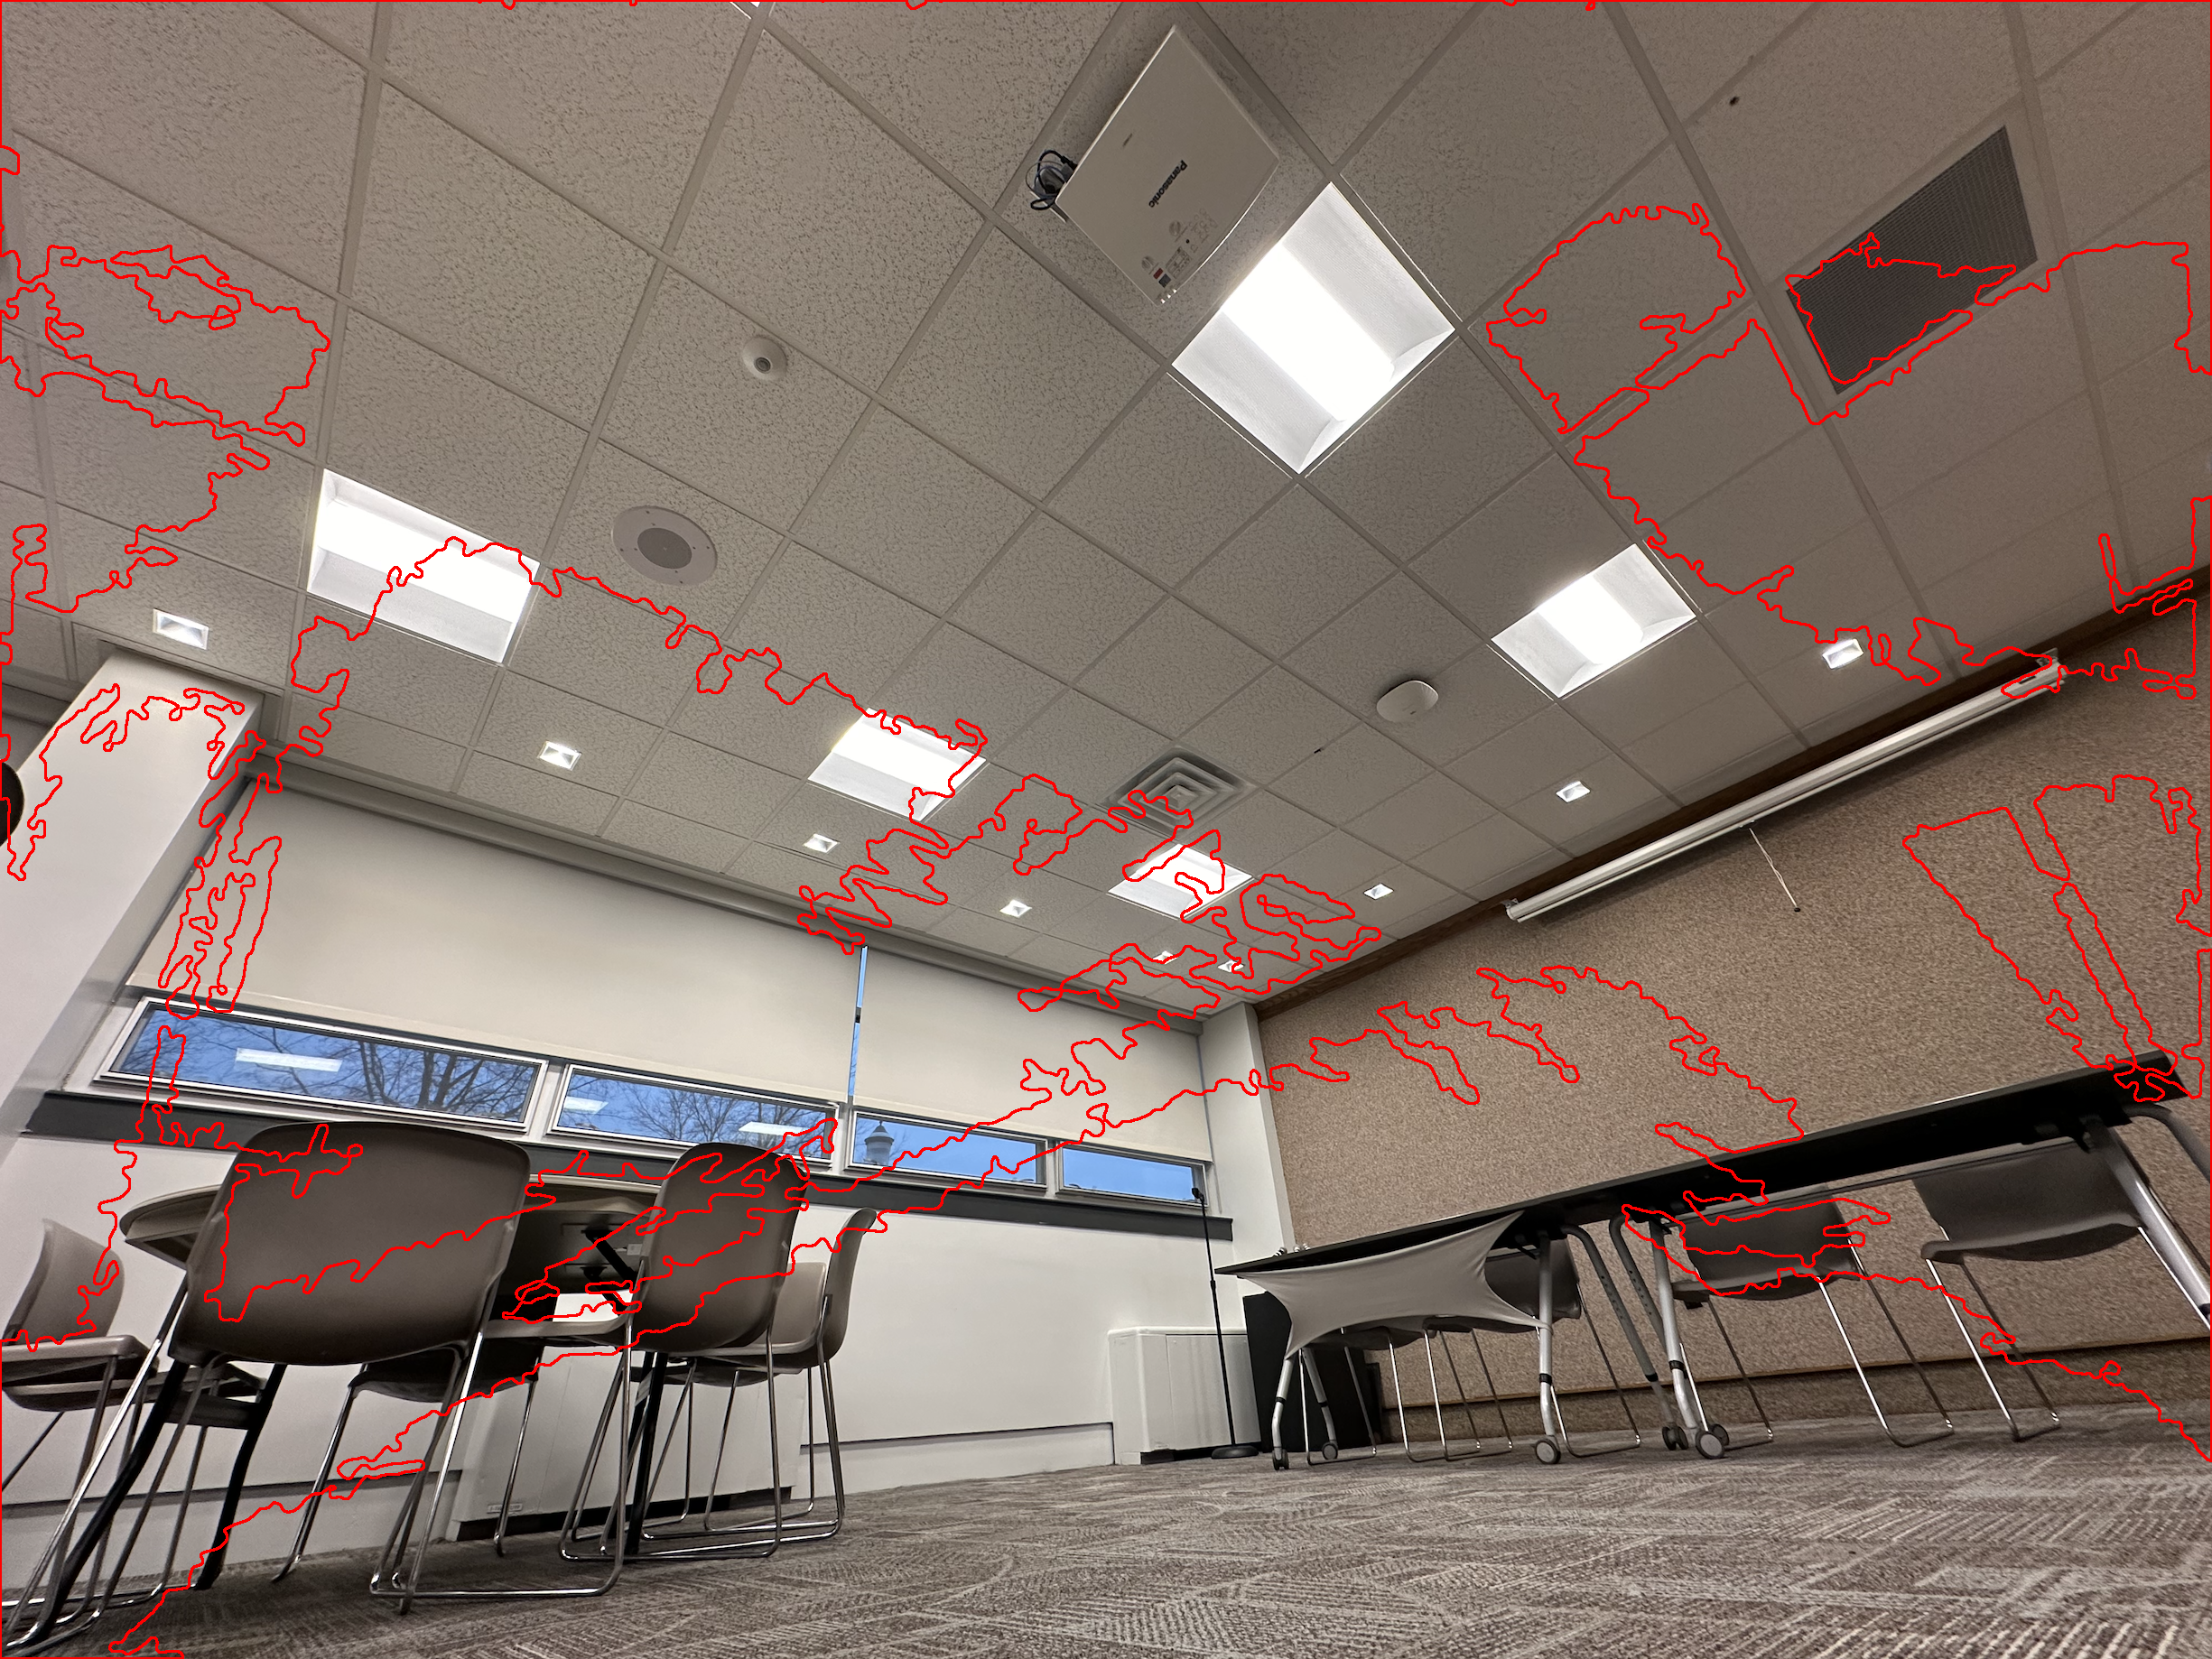
\includegraphics[width=0.8\textwidth]{3vp Most Converged Area.png}
    \caption{3VP Perspective View Vanishing Point Possibility Space}
    \label{fig: 3VP perspective view Vanishing point possibility space}
\end{figure}

\begin{figure}[H]
    \centering
    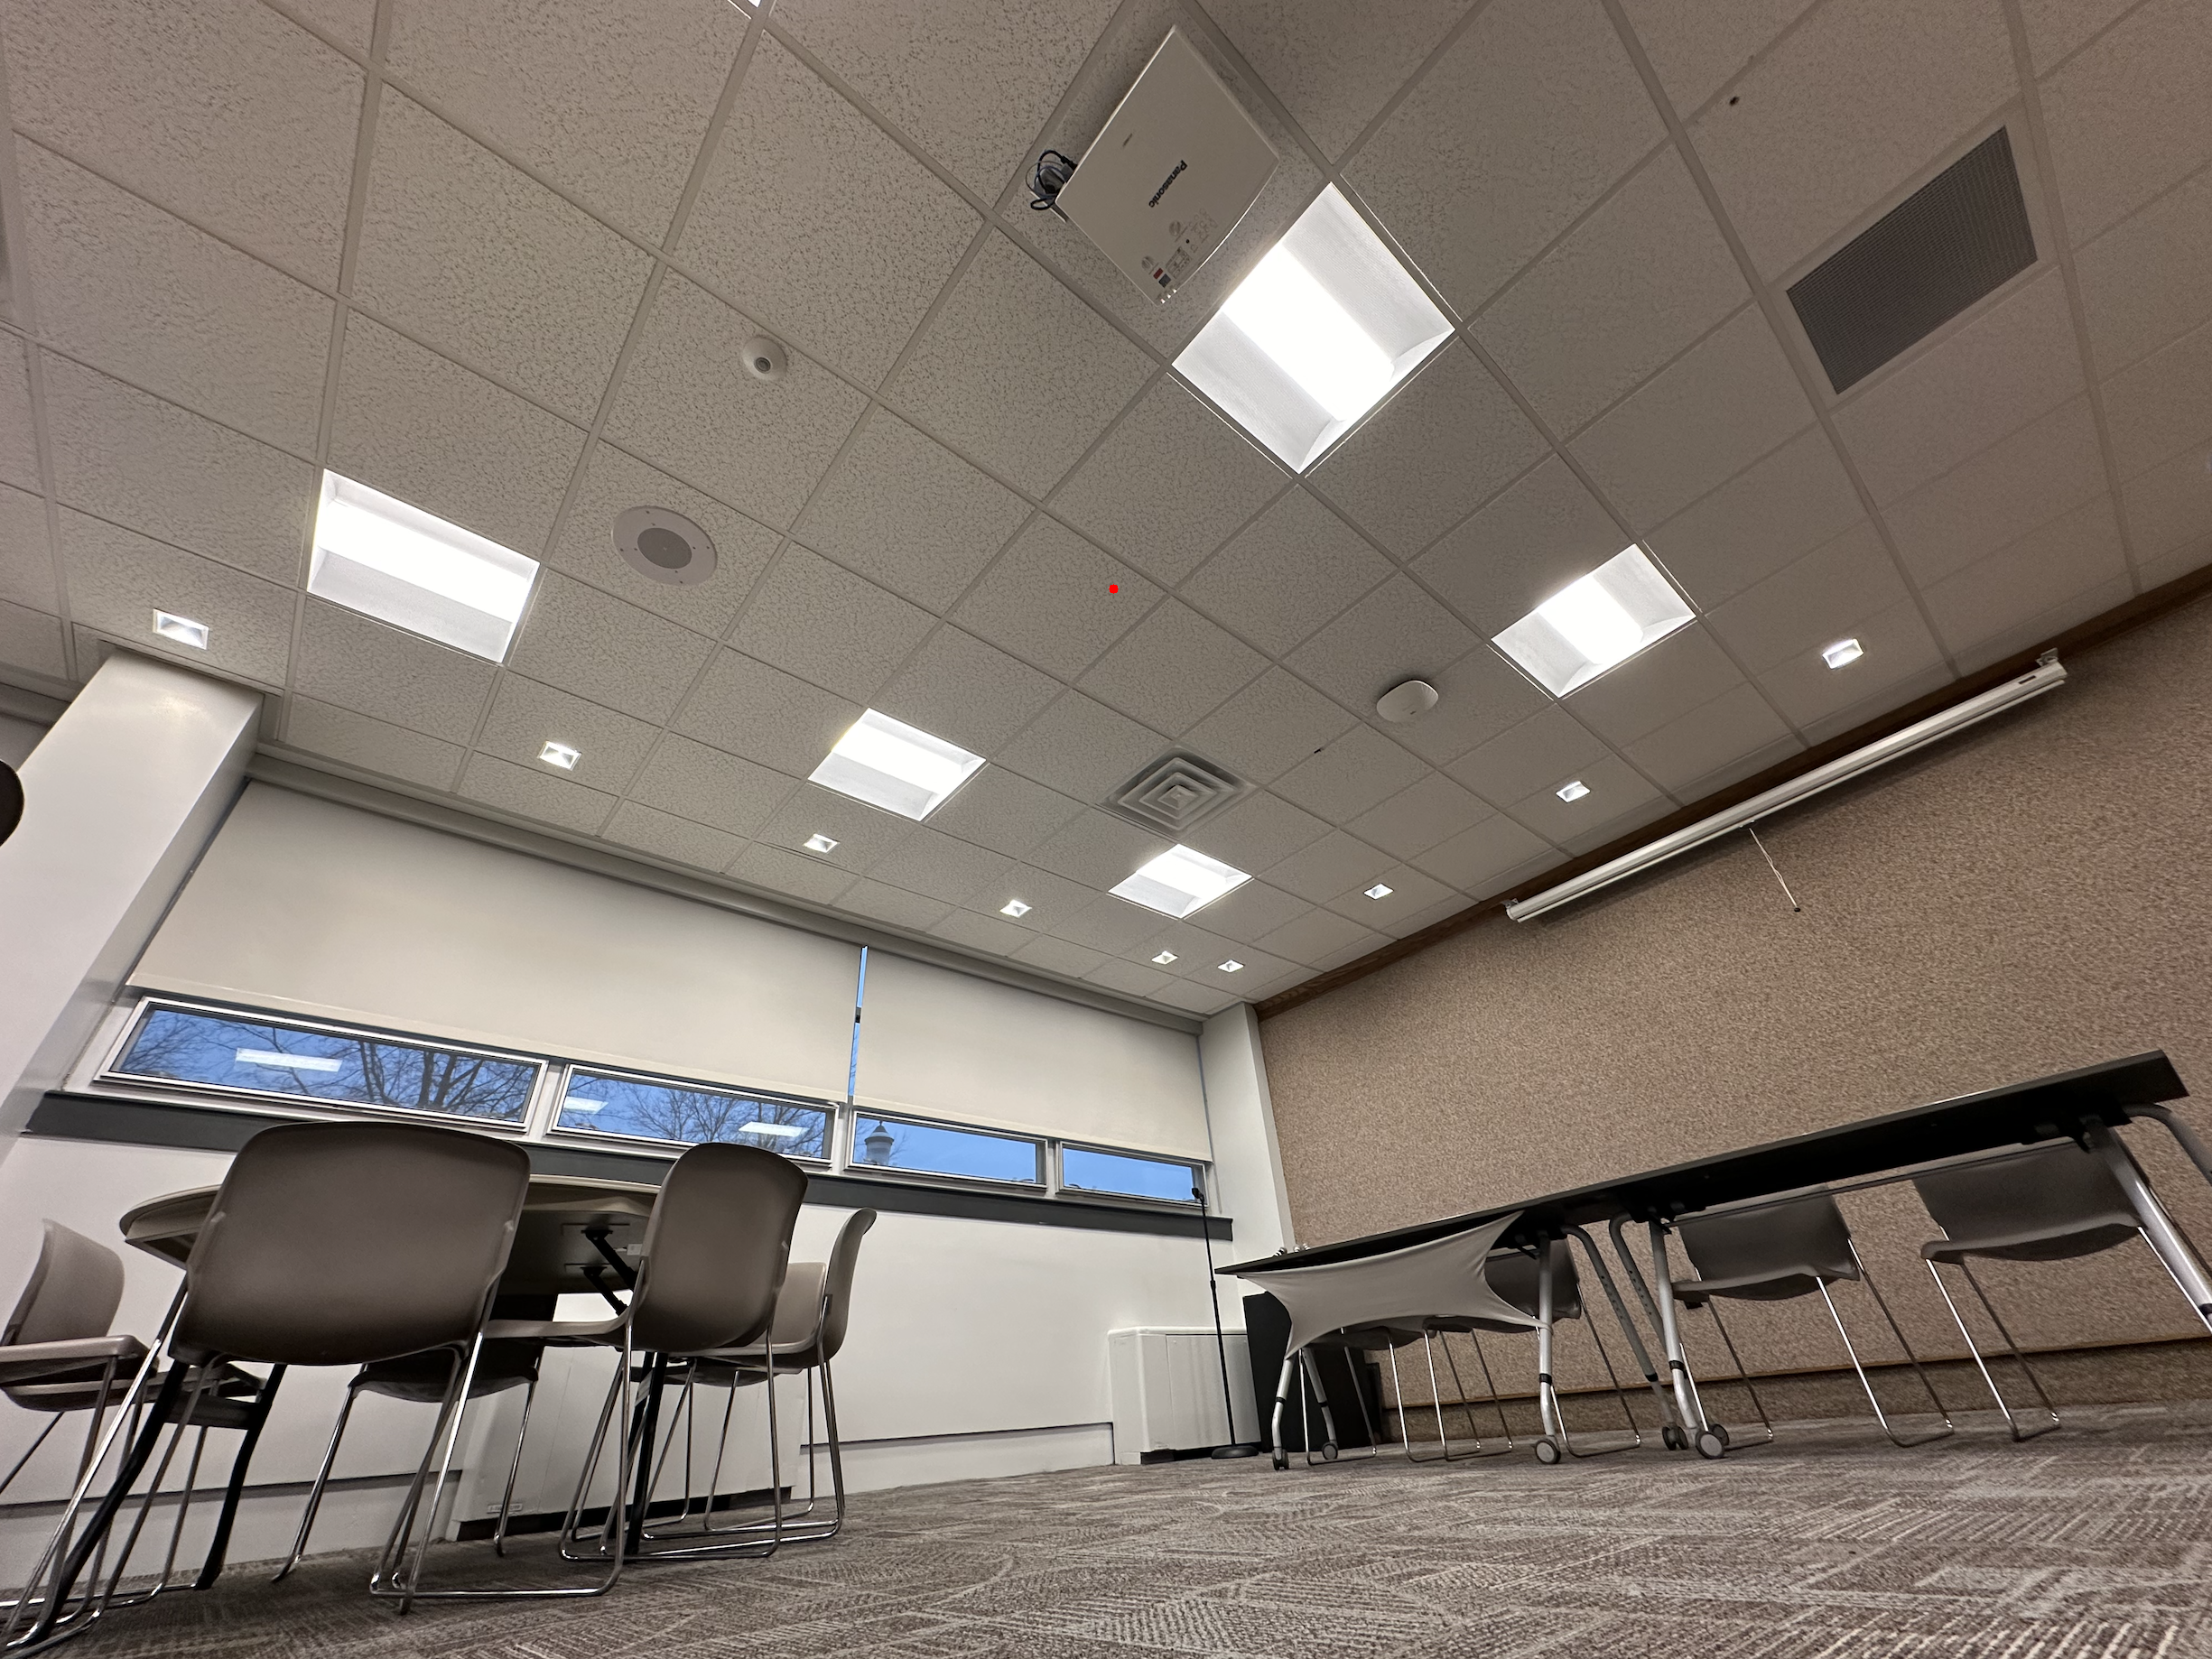
\includegraphics[width=0.8\textwidth]{3vp Centroid of Most Converged Area.png}
    \caption{3VP Perspective View Weighted Vanishing Point}
    \label{fig: 3VP perspective view Weighted Vanishing Point}
\end{figure}

\subsection{Person and Pose Detection}

\begin{figure}[H]
    \centering
    \includegraphics[width=1.0\textwidth]{1vp person.jpg}
    \caption{Person Standing in a 1VP Perspective View Scene}
    \label{fig: Person standing in a 1VP perspective view Scene}
\end{figure}

\begin{figure}[H]
    \centering
    \includegraphics[width=1.0\textwidth]{1vp person pose.png}
    \caption{Pose Marked Person Standing in a 1VP Perspective View Scene}
    \label{fig: Pose marked person standing in a 1VP perspective view Scene}
\end{figure}


Figure \ref{fig: Person standing in a 1VP perspective view Scene} and Figure \ref{fig: Pose marked person standing in a 1VP perspective view Scene} showcase the a person standing in a 1VP perspective view scene. These images are a part of a video stream that the implementation was tested on. Figure \ref{fig: Pose marked person standing in a 1VP perspective view Scene} shows the same person with his pose marked over him.\newline

\begin{figure}[H]
    \centering
    \includegraphics[width=1.0\textwidth]{1vp partial person.jpg}
    \caption{Partially Visible Person Standing in a 1VP Perspective View Scene}
    \label{fig: Partially visible Person standing in a 1VP perspective view Scene}
\end{figure}

Figure \ref{fig: Partially visible Person standing in a 1VP perspective view Scene} is from the same video stream as Figure \ref{fig: Person standing in a 1VP perspective view Scene} however here the person is partially occluded behind a desk. Figure \ref{fig: Boundary and pose detected of a partially occluded person} shows the dynamic window created around the person. The person also has a bounding box created around them and their predicted pose marked over them to properly calculate their coordinates.\newline

\begin{figure}[H]
    \centering
    \includegraphics[width=1.0\textwidth]{1vp partial person pose.png}
    \caption{Boundary and Pose Detected of a Partially Occluded Person}
    \label{fig: Boundary and pose detected of a partially occluded person}
\end{figure}

\subsection{Coordinate Calculation and Tracking}

\begin{figure}[H]
    \centering
    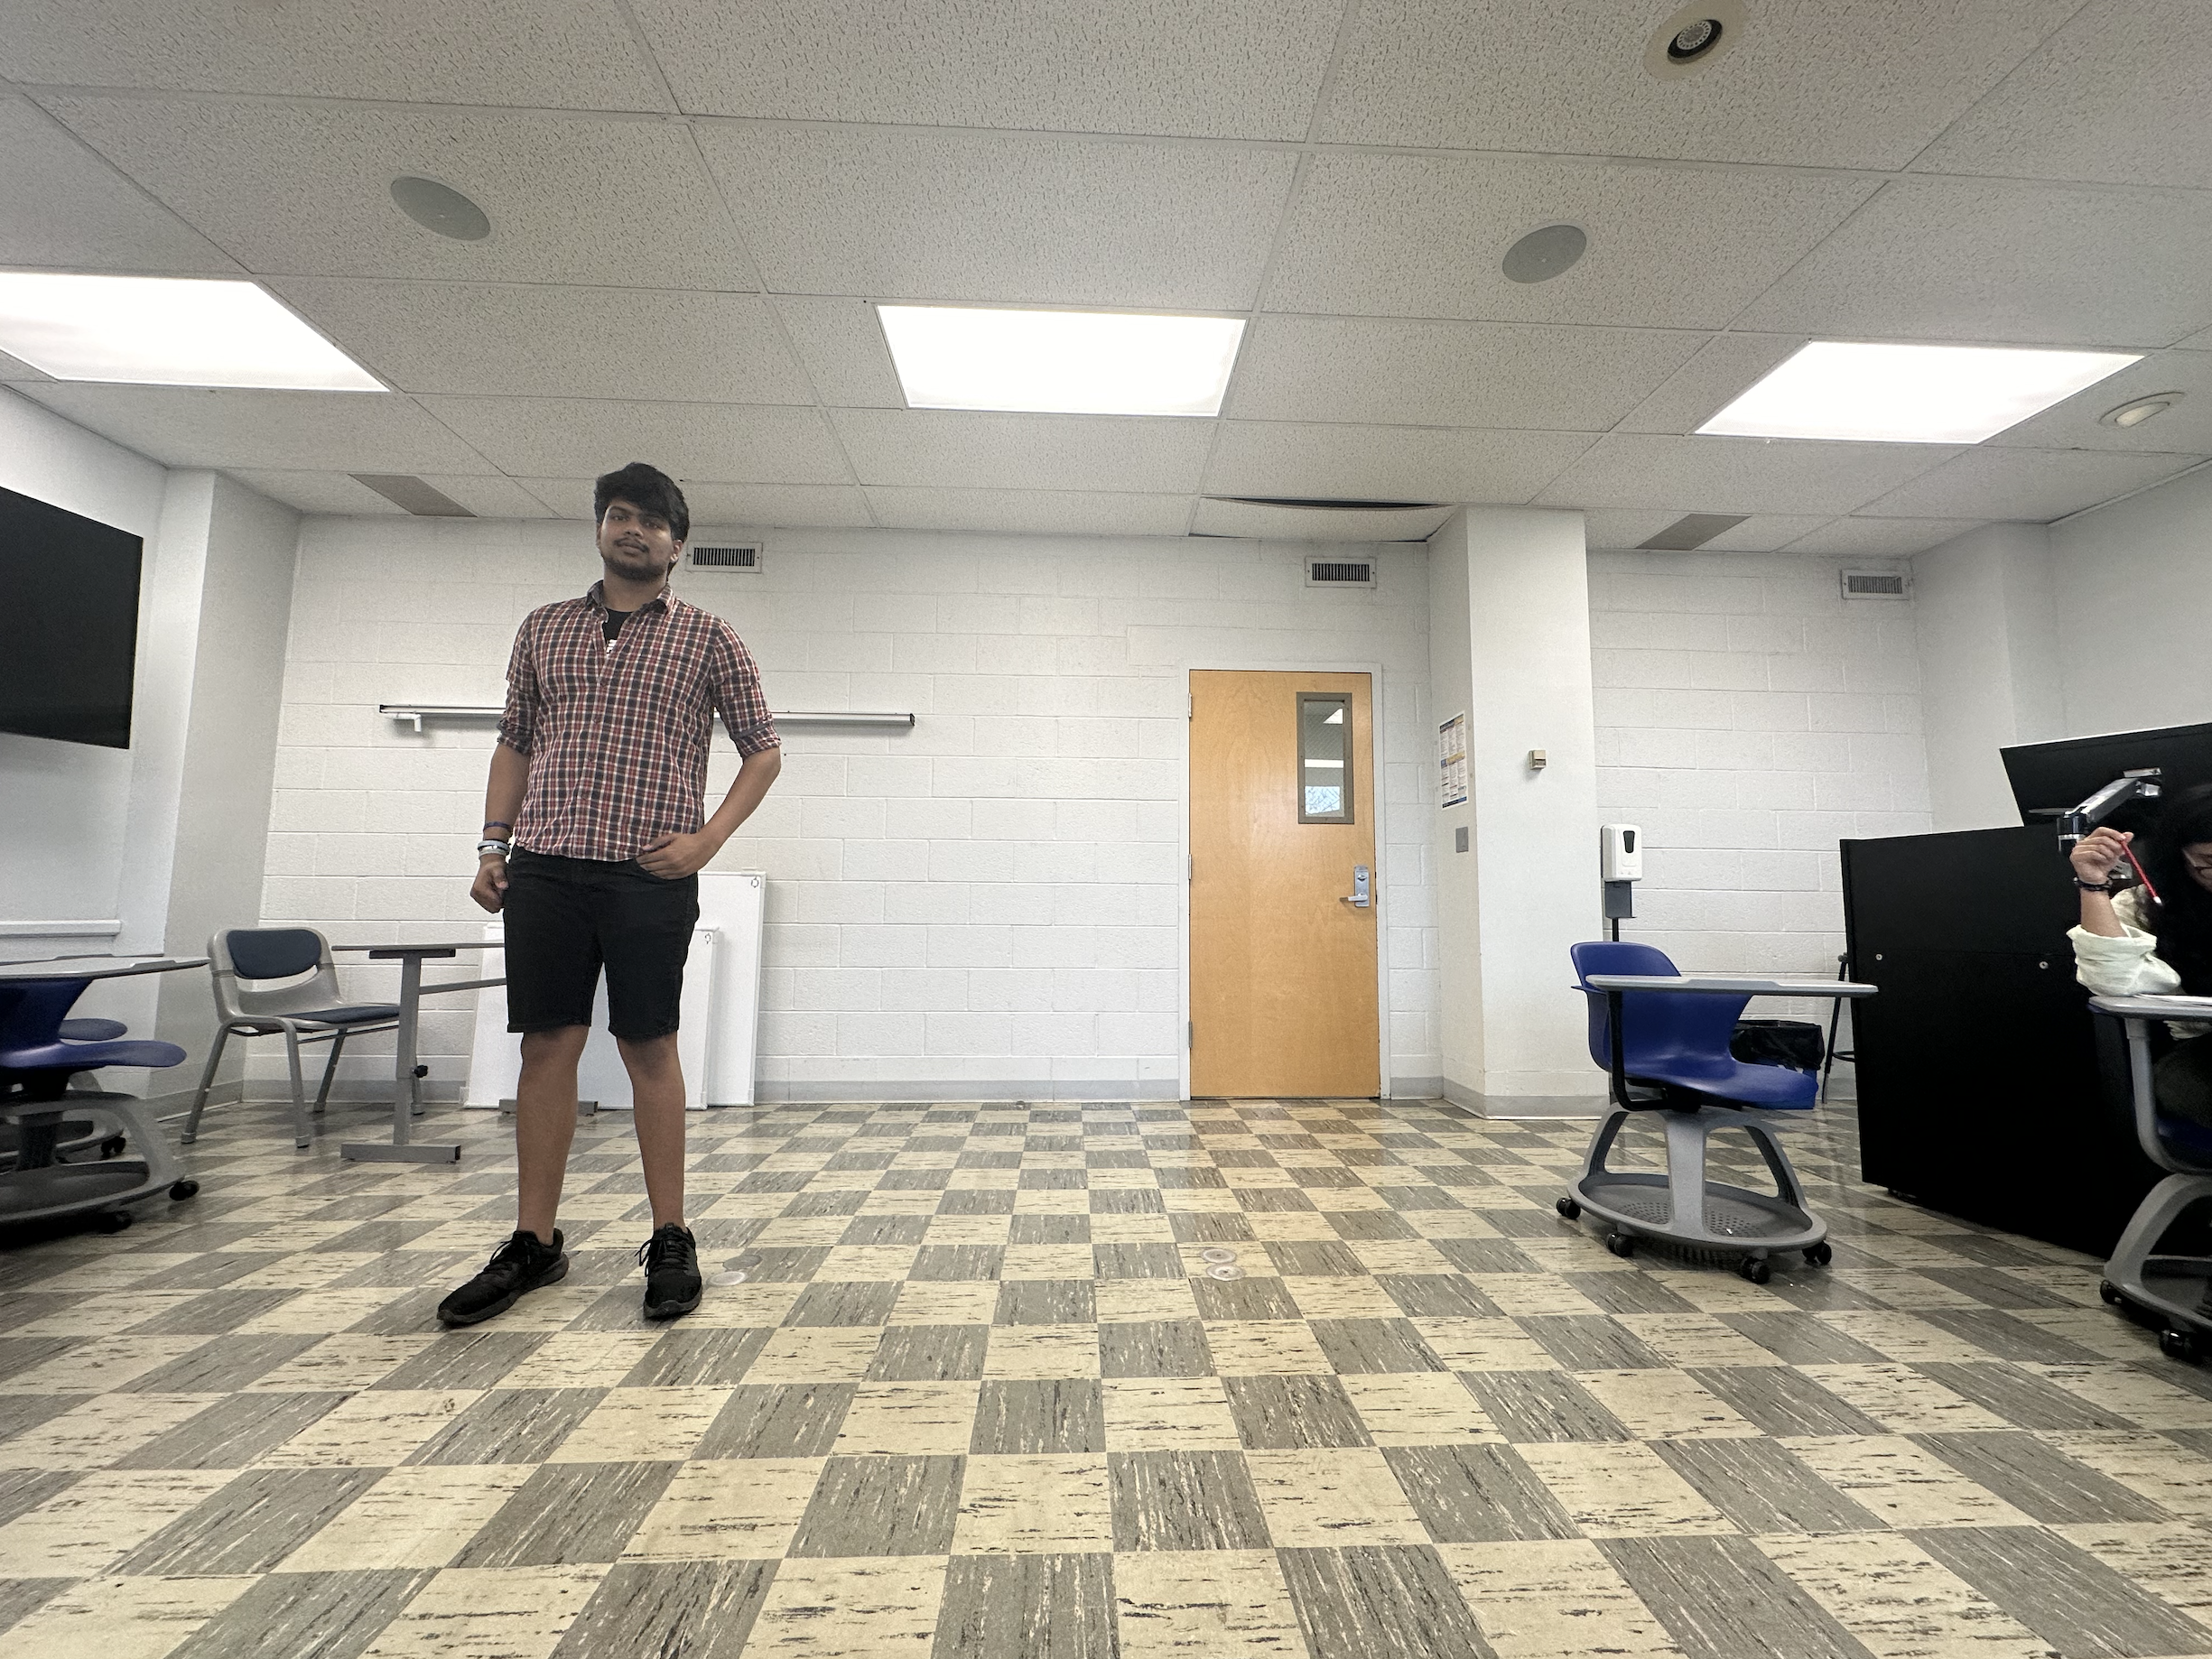
\includegraphics[width=0.8\textwidth]{vineet.png}
    \caption{A Tall Person in a Room}
    \label{fig: A tall person in a room}
\end{figure}

\begin{figure}[H]
    \centering
    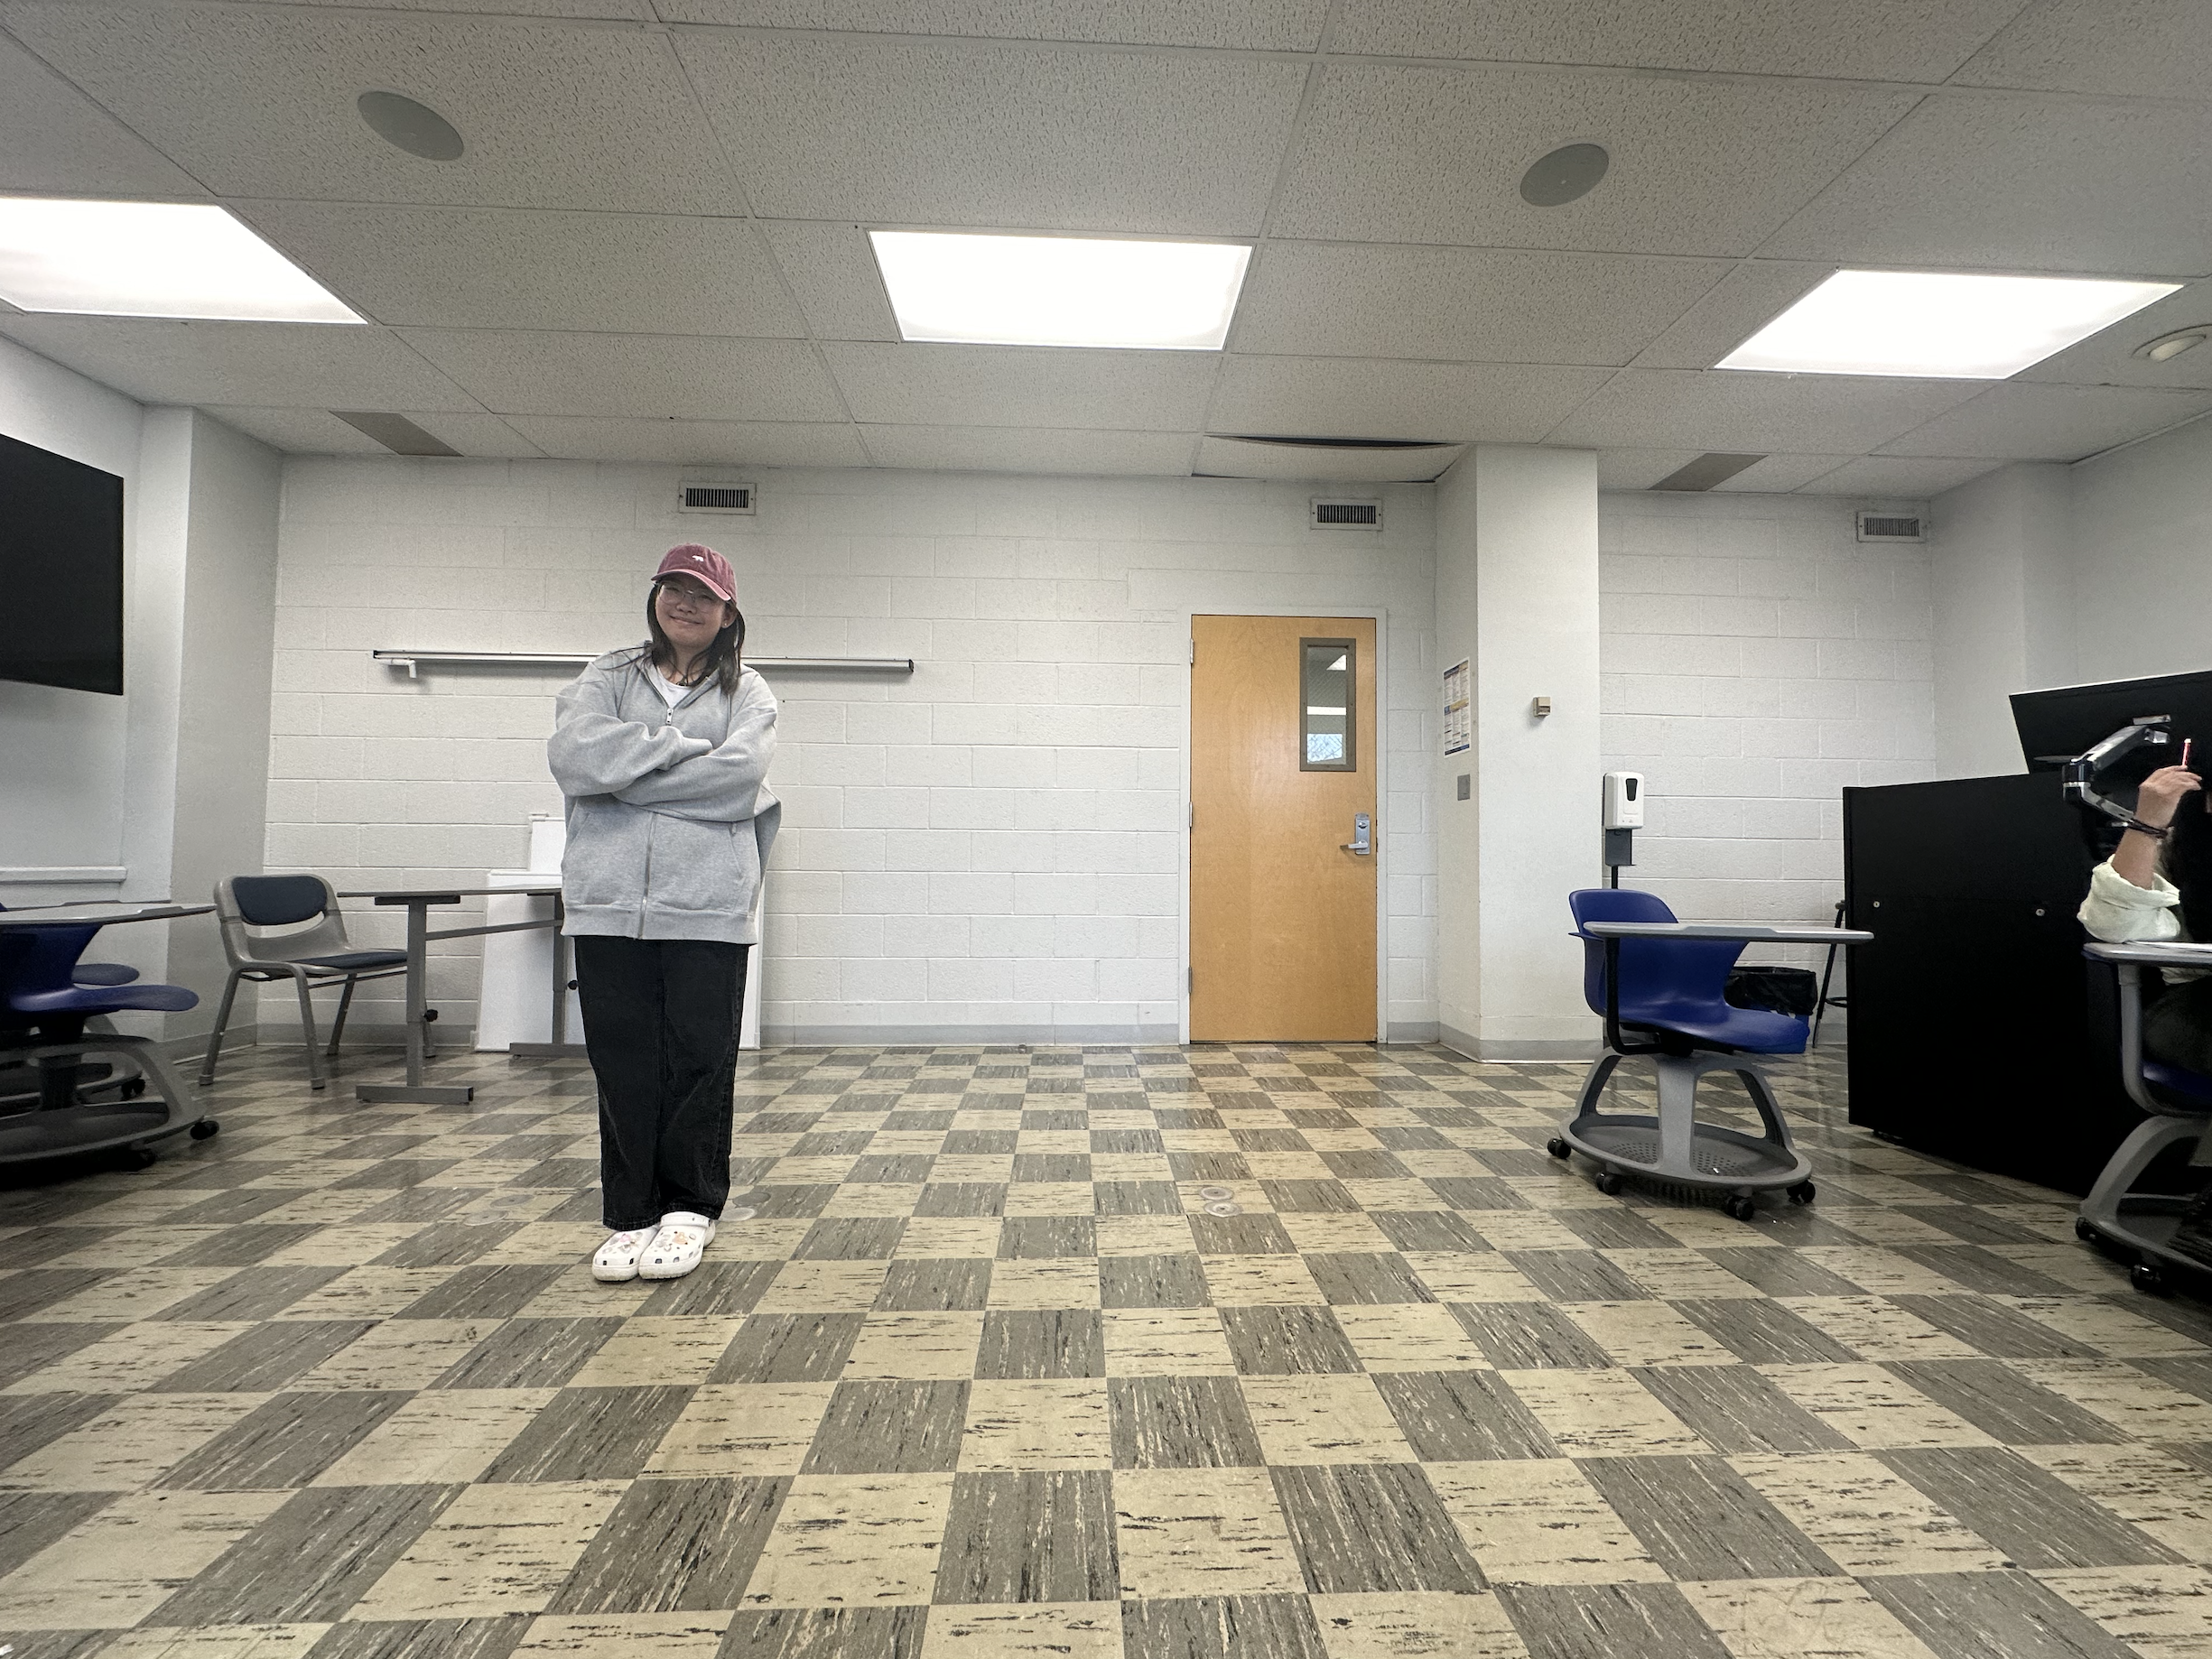
\includegraphics[width=0.8\textwidth]{rexha.png}
    \caption{A Short Person in a Room}
    \label{fig:A short person in a room}
\end{figure}

\begin{figure}[H]
    \centering
    \includegraphics[width=0.8\textwidth]{vineet line.jpeg}
    \caption{Tall Person Coordinate Calculation}
    \label{fig:Tall person coordinate calculation}
\end{figure}

\begin{figure}[H]
    \centering
    \includegraphics[width=0.8\textwidth]{rexha line.jpeg}
    \caption{Short Person Coordinate Calculation}
    \label{fig:Short person coordinate calculation}
\end{figure}

Figure \ref{fig: A tall person in a room} and Figure \ref{fig:A short person in a room} show two people with a significant height difference standing at the same position in the same scene, and Figure \ref{fig:Tall person coordinate calculation} and Figure \ref{fig:Short person coordinate calculation} show the same projection line created for both people. The images and the videos for the testing of the thesis were captured by hand and not a fixed camera with a tripod, therefore there exists a little difference in the field of view of different images and a little camera shake in the videos. These minor imperfections caused by human error present themselves in the form of a reduction of precision and accuracy to a small degree. As long as we can ignore minor errors in the coordinates if they are within an acceptable range, the method yields promising results.\newline




\chapter{Conclusion and Future Work}

Object tracking and Coordinate detection is a task with a lot of use cases. However traditional methods for doing so either work only in the image space or need a lot of equipment and preparation to properly work. Monocular vision images and videos are very common and easy to capture. However, they lack the inherent depth information that comes with having specialized equipment and hence, they are not used for the purposes of tracking people/objects in a 3D space. However, using the power of vanishing points along with perspective views the approach provided in Chapter 3 gives an elegant solution to this problem and opens up an opportunity to use the previously unusable data for the task at hand. The results shown in Chapter 4 also Show that the method provided in Chapter 3 holds great potential to be widely used and reduce the need for specialized equipment.\newline

Even though the results are promising and the method shows potential, there still is scope for improvement, particularly in the recognition and the mapping of the room. Complex scenes in images and the presence of texture on surfaces make it harder for the algorithm to efficiently place the person detected in the image. The accuracy of the calculation of the coordinates and tracking is also dependent on how efficient the model being used for subject detection is. Since the method has some dependencies there is a little bit of a journey that the programs need to make before the method can effectively be used to replace the current methods.\newline

\newpage
% Bibliography
% Include your bibliography file here
\addcontentsline{toc}{chapter}{Bibliography}
\bibliographystyle{unsrt}
\bibliography{reference} 

\end{document}